\documentclass[12pt,a4paper,oneside,openright]{report}
\let\openright=\cleardoublepage



%%% Choose a language %%%

\newif\ifEN
\ENtrue   % uncomment this for english
%\ENfalse   % uncomment this for czech

%%% Configuration of the title page %%%

\def\ThesisTitleStyle{mff} % MFF style
%\def\ThesisTitleStyle{cuni} % uncomment for old-style with cuni.cz logo
%\def\ThesisTitleStyle{natur} % uncomment for nature faculty logo

\def\UKFaculty{Faculty of Mathematics and Physics}
%\def\UKFaculty{Faculty of Science}

\def\UKName{Charles University in Prague} % this is not used in the "mff" style

% Thesis type names, as used in several places in the title
%\def\ThesisTypeTitle{\ifEN BACHELOR THESIS \else BAKALÁŘSKÁ PRÁCE \fi}
\def\ThesisTypeTitle{\ifEN MASTER THESIS \else DIPLOMOVÁ PRÁCE \fi}
%\def\ThesisTypeTitle{\ifEN RIGOROUS THESIS \else RIGORÓZNÍ PRÁCE \fi}
%\def\ThesisTypeTitle{\ifEN DOCTORAL THESIS \else DISERTAČNÍ PRÁCE \fi}
%\def\ThesisGenitive{\ifEN bachelor \else bakalářské \fi}
\def\ThesisGenitive{\ifEN master \else diplomové \fi}
%\def\ThesisGenitive{\ifEN rigorous \else rigorózní \fi}
%\def\ThesisGenitive{\ifEN doctoral \else disertační \fi}
%\def\ThesisAccusative{\ifEN bachelor \else bakalářskou \fi}
\def\ThesisAccusative{\ifEN master \else diplomovou \fi}
%\def\ThesisAccusative{\ifEN rigorous \else rigorózní \fi}
%\def\ThesisAccusative{\ifEN doctoral \else disertační \fi}



%%% Fill in your details %%%

% (Note: \xxx is a "ToDo label" which makes the unfilled visible. Remove it.)
\def\ThesisTitle{Efficient hyperparameter optimization}
\def\ThesisAuthor{Bc.~Jiří Krejčí}
\def\YearSubmitted{2024}

% department assigned to the thesis
\def\Department{Department of Theoretical Computer Science and Mathematical Logic}
% Is it a department (katedra), or an institute (ústav)?
\def\DeptType{Department}

\def\Supervisor{doc.~Mgr.~Martin Pilát,~Ph.D.}
\def\SupervisorsDepartment{Department of Theoretical Computer Science and Mathematical Logic}

% Study programme and specialization
\def\StudyProgramme{Computer Science}
\def\StudyBranch{Artificial Intelligence (IUIP)}

\def\Dedication{%
I am grateful for the support and patience of my family, my partner, and my friends on this arduous journey. I also appreciate all the support and great advice of my supervisor Martin Pilát. Thank you.

A special mention goes to the e-INFRA CZ project (ID:90254), supported by the Ministry of Education, Youth and Sports of the Czech Republic, for providing the computational resources.
}

\def\AbstractEN{%
Hyperparameter optimization significantly impacts model performance and substantial effort went into the development of robust and efficient algorithms for this task. Our research found that several new algorithms utilizing partial evaluations have been published recently. However, it is not clear from the literature how the algorithms perform in various scenarios. In this thesis, we compared the leading algorithms through experiments on diverse tasks, including tabular benchmarks and real-world deep-learning problems, with a special focus on healthcare datasets. The results show that the recent multi-fidelity techniques outperform random search. Nevertheless, no single algorithm consistently excelled across all problems, highlighting the need for ongoing comparison studies in hyperparameter optimization.
}

\def\AbstractCS{%
Ladění hyperparametrů má značný vliv na vlastnosti výsledného modelu a vývoji robustních a efektivních algoritmů pro tuto úlohu bylo věnováno velké úsilí. Nedávno bylo vyvinuto několik nových algoritmů využívajících částečných vyhodnocení optimalizované funkce. Z literatury nicméně není zřejmé, jak si tyto algoritmy vedou na rozmanitých problémech. V této diplomové práci jsme experimentálně srovnali aktuální algoritmy pro ladění hyperparametrů v mnoha úlohách. Tyto úlohy se skládaly z tabulárních benchmarků a reálných úloh hlubokého učení, včetně datových sad z oblasti zdravotnictví. Výsledky ukazují, že nedávné multi-fidelity techniky dosahují lepších výsledků než náhodné prohledávání. Přesto však žádný algoritmus nepodával konzistentně nejlepší výkon ve všech problémech, což zdůrazňuje potřebu průběžných srovnávacích studií v oblasti optimalizace hyperparametrů.
}

% 3 to 5 keywords (recommended), each enclosed in curly braces.
% Keywords are useful for indexing and searching for the theses by topic.
\def\Keywords{%
{deep learning} {hyperparameter optimization} {Bayesian optimization} {multi-fidelity}
}

% If your abstracts are long and do not fit in the infopage, you can make the
% fonts a bit smaller by this setting. (Also, you should try to compress your abstract more.)
% Alternatively, consider increasing the size of the page by uncommenting the
% geometry modification in thesis.tex.
\def\InfoPageFont{}
%\def\InfoPageFont{\small}  %uncomment to decrease font size



\usepackage[a-2u]{pdfx}

\ifEN\else\usepackage[czech,shorthands=off]{babel}\fi

% See https://en.wikipedia.org/wiki/Canons_of_page_construction before
% modifying the size of printable area. LaTeX defaults are great.
% If you feel it would help anything, you can enlarge the printable area a bit:
%\usepackage[textwidth=390pt,textheight=630pt]{geometry}
% The official recommendation expands the area quite a bit (looks pretty harsh):
%\usepackage[textwidth=145mm,textheight=247mm]{geometry}

%%% TYPICAL FONT CHOICES (uncomment what you like) %%%
% Recommended combo: Libertinus (autoselects Biolinum for sans) and everything
% else (math+tt) comes from Latin Modern)
\usepackage{cmap} % to be PDF/A compatible
\usepackage[T1]{fontenc}
\usepackage{lmodern}
\usepackage[mono=false]{libertinus}

% For the "classic" LaTeX fonts (very good for pure math theses), simply
% comment out the libertinus package above.

% IBM Plex font suite: nice, but requires us to fine-tune the sizes and does
% not directly support small caps (\textsc):
%\usepackage[usefilenames,RM={Scale=0.88},SS={Scale=0.88},SScon={Scale=0.88},TT={Scale=0.88},DefaultFeatures={Ligatures=Common}]{plex-otf}

% TeX Gyre combo (Pagella+Heros+Cursor)
%\usepackage{fontspec}
%\setmainfont{TeX Gyre Pagella}
%\setsansfont{TeX Gyre Heros}
%\setmonofont{TeX Gyre Cursor}

% some useful packages
\usepackage{microtype}
\usepackage{amsmath,amsfonts,amsthm,bm}
\usepackage{graphicx}
\usepackage{xcolor}
\usepackage{booktabs}
\usepackage{caption}
\usepackage{subcaption}
%\usepackage{float}
\usepackage{siunitx}
\usepackage{floatrow}

\usepackage{subfiles}
\usepackage{interval}

% Bibliography formatting.
% CHECK THE REQUIREMENTS OF YOUR DEPARTMENT AND FACULTY ON THE CITATION FORMAT!
%
% These are relatively "safe" default options that most people use:
\usepackage[natbib,style=numeric,sorting=none]{biblatex}
% alternative with alphanumeric citations (more informative than numbers, and
% more common in computer science journals):
%\usepackage[natbib,style=alphabetic]{biblatex}
%
% ALTERNATIVES THAT CONFORM TO ISO690
% ISO690 is not the greatest citation format ever, but may be formally
% required at Charles University, depending on your faculty and department.
%\usepackage[natbib,style=iso-numeric,sorting=none]{biblatex}
%\usepackage[natbib,style=iso-alphabetic]{biblatex}
% You might want to add extra options such as `maxbibnames=6,maxcitenames=2`
% here to further conform to some of the formatting requirements (see below for
% details). Again, consult your faculty rules.
%
% Additional option choices:
%  - add `giveninits=true` to typeset "E. A. Poe" instead of full Edgar Allan
%  - `terseinits=true` additionaly shortens it to nature-like "Poe EA"
%  - add `maxnames=10` to limit (or loosen) the maximum number of authors in
%    bibliography entry before shortening to `et al.` (useful when referring to
%    book collections that may have hundreds of authors)
%  - use `maxcitenames=2` to finetune the amount of authors listed in text-cite
%    commands (\citet). Corresponding option that only affects the bibliography
%    is `maxbibnames=10`.
%  - `sorting=none` causes the bibliography list to be ordered by the order of
%    citation as they appear in the text, which is usually the desired behavior
%    with numeric citations. Additionally you can use a style like
%    `numeric-comp` that compresses the long lists of citations such as
%    [1,2,3,4,5,6,7,8] to simpler [1--8]. This is especially useful if you plan
%    to add tremendous amounts of citations, as usual in life sciences and
%    bioinformatics.
%  - if you don't like the "In:" appearing in the bibliography, use the
%    extended style (`ext-numeric` or `ext-alphabetic`), and add option
%    `articlein=false`.
%
% possibly reverse the names of the authors with the default styles:
%\DeclareNameAlias{default}{family-given}

% load the file with bibliography entries
\addbibresource{refs.bib}

% remove this if you won't use fancy verbatim environments
\usepackage{fancyvrb}

% remove this if you won't typeset TikZ graphics
\usepackage{tikz}
\usetikzlibrary{positioning, shapes.geometric, arrows.meta} %add libraries as needed (shapes, decorations, ...)

% remove this if you won't typeset any pseudocode
\usepackage[noend]{algpseudocode}
\usepackage{algorithm}

% remove this if you won't list any source code
\usepackage{listings}


\hypersetup{unicode}
\hypersetup{breaklinks=true}

\usepackage[noabbrev]{cleveref}

\input{macros} % use this file for various custom definitions


\begin{document}

\include{title}

\tableofcontents


\chapwithtoc{Introduction}
% Zadani
% Mnoho metod strojového učení je citlivých na nastavení hyper-parametrů. V posledních letech se rychle rozvíjí metody pro ladění tohoto nastavení. Většina existujících metod je ale velmi výpočetně náročná, což komplikuje jejich reálné nasazení. Zároveň chybí podrobnější porovnání výkonnosti jednotlivých metod. Cílem práce je porovnat existující metody pro ladění hyper-parametrů a navrhnout nové metody s ohledem nejen na kvalitu nalezených nastavení, ale také na dobu běhu.

% Student nastuduje dostupné metody a knihovny pro ladění hyper-parametrů metod strojového učení. Vybrané metody mezi sebou porovná a na základě získaných informací implementuje metody nové, které budou uvažovat jak rychlost ladění tak kvalitu nalezených řešení.

 %Establish the importance of the field
 %   1 Establish the importance of this research topic
 %         Hyperparameter optimization is important because
%
 %   2 Provide general background information
 %       The two most common approaches to hyperparameter tuning are by hand, or using a random search.
 %   3 Provide more detailed background information
 %   4 Describe the general problem area or the current research focus of the field
 %Previous or current research
 %   5 Provide a transition between the general problem area and the literature review
 %   6 Provide a brief overview of key research projects in this area
 %Locate a gap in research
 %   7 Describe a gap in the research
 %Describe the present paper
 %   8 Describe the paper itself
 %   9 Give details about the methodology reported in the paper
 %   10 Announce the findings

% Introduction should answer the following questions, ideally in this order

% What is the nature of the problem the thesis is addressing?
Hyperparameter optimization is an important step in the machine learning workflow that can have a striking effect on model generalization and performance. Historically, the most prevalent approaches to hyperparameter optimization were tuning the hyperparameters manually, using a random search, or a grid search. A breakthrough in the field was the adaptation of Bayesian optimization~\cite{mockus1974bayesian,snoek2012practical}, which uses probabilistic models to predict the performance of hyperparameter configurations to make an informed decision about which configuration to evaluate next. Nevertheless, as the complexity of machine learning models has increased rapidly in recent years, not even Bayesian optimization alone might be feasible for many tasks. The next step seems to be the multi-fidelity hyperparameter tuning, which makes use of cheap but unreliable evaluations, often combined with Bayesian optimization.

% What is the common approach for solving that problem now?
% How this thesis approaches the problem?
% What are the results? Did something improve?
We conduct a literature survey on state-of-the-art hyperparameter optimization methods. Additionally, we examine the underlying principles of these methods, explaining the most important ideas and their practical implications. Our research found that limited performance comparisons of hyperparameter optimization algorithms were available. Therefore, instead of developing a new algorithm, we carried out experiments to compare the most promising algorithms across various tasks. These tasks include tabular benchmarks as well as real-world deep-learning problems. In addition to the usual image datasets, we chose two datasets from the healthcare domain, too. The results of the experiments confirm that multi-fidelity techniques are superior to random search, but no single algorithm consistently outperforms others across all tasks.

% that will do well on any problem?
% add more information about the multi-fidelity
% add more about the experiments, include healthcare domain

% What can the reader expect in the individual chapters of the thesis?
The thesis is divided into four chapters. In Chapter~1 we introduce key concepts and definitions that will be used throughout the thesis. These include a brief introduction to machine learning, a formal definition of the hyperparameter optimization problem, and hyperparameter optimization techniques including Bayesian optimization. In Chapter~2 we explore multi-fidelity optimization techniques in depth. Chapter~3 discusses the methodology, which includes the design of the experiments and how the collected data from the experiments are processed. In Chapter~4 we present the results and interpret them in the discussion.


% Expected length of the introduction is between 1--4 pages. Longer introductions may require sub-sectioning with appropriate headings --- use \texttt{\textbackslash{}section*} to avoid numbering (with section names like `Motivation' and `Related work'), but try to avoid lengthy discussion of anything specific. Any ``real science'' (definitions, theorems, methods, data) should go into other chapters.
% \todo{You may notice that this paragraph briefly shows different ``types'' of `quotes' in TeX, and the usage difference between a hyphen (-), en-dash (--) and em-dash (---).}

% It is very advisable to skim through a book about scientific English writing before starting the thesis. I can recommend `\citetitle{glasman2010science}' by \citet{glasman2010science}.
\chapter{Background}
% Maybe split into two chapters?

\label{chap:refs}

\section{Machine learning basics}
% TODO: Formulation could be better.
Our goal is to optimize hyperparameters, but before we introduce the main topic, we need to specify the context --- machine learning. We include this chapter to introduce the notation and to give readers some intuition for the machine learning algorithms and models underlying hyperparameter optimization in this thesis. Readers familiar with machine learning, and with deep learning in particular, can skip this section and start directly with hyperparameter optimization in Section~\ref{sec:hpo}. The material in this section is covered by the~\citetitle{Goodfellow-et-al-2016} book~\cite{Goodfellow-et-al-2016}. First, we will introduce the task of supervised machine learning, how the dataset is commonly split, and the function that is optimized in order to train the model. Then we will briefly introduce deep learning and a couple of frequently used architectures. Finally, we will end with an overview of the optimization algorithm behind neural networks.

% In general, machine learning is the ability of an AI system to acquire its own knowledge by extracting patterns from raw data. In the last decade, one particular class of machine learning algorithms took over --- deep learning.

%Before we get to hyperparameters and optimization, we will revisit and define key concepts from machine learning so that it is clear what machine learning models we use and why.


% Briefly revisit deep neural networks and ML

% Machine learning applications - should I introduce machine learning in general? I think everyone has to know

\subsection{Supervised machine learning}
% Dataset, labeled examples, classification vs regression
Let $\mathcal{D}$ be a labeled dataset, consisting of examples generated independently from a data-generating distribution. Each example $(x^{(i)}, \  y^{(i)})$ consist of a feature vector $x^{(i)}\in \mathcal{X}$ and its label $y^{(i)}\in \mathcal{Y}$. Depending on the labels, we distinguish classification and regression. In classification, the labels are from a finite set, while in regression the labels are real numbers. The goal of supervised learning is to train a model using the examples from the dataset $\mathcal{D}$ so that it generalizes well to data from the data-generating distribution. Simply put, we want the model to correctly predict the labels on unseen data. We assume the unseen data come from the same data-generating distribution so that the model can use the learned patterns for the task.  % Generalization error

% Generalization, train, val, test split
Since the goal is for the model to generalize well, we need to estimate the generalization error in the training and model selection process on unseen data. It is a best practice to split the dataset into $\mathcal{D}_{train}, \  \mathcal{D}_{val}, \mathcal{D}_{test}$. We use $\mathcal{D}_{train}$ for the training of the model, $\mathcal{D}_{val}$ for the estimate of the generalization error during development, and $\mathcal{D}_{test}$ for the final evaluation. A separate test set is needed for the final evaluation because the validation set has already been used to choose the best model, which means there is a bias in the estimate. As we will see, using a hyperparameter optimization tool introduces yet another optimization layer, meaning we should do a similar split even for the outer optimization of hyperparameters.


% Training - minimizing the loss function
We train machine learning algorithms by minimizing the loss function on the training data. Two loss functions are used most commonly. For regression, the mean square error of $N$ examples is computed as $$ MSE=\frac{1}{N} \sum_{i=1}^{N} (f(x^{(i)});\theta )-y^{(i)})^2.$$

% Cross entropy loss, MSE loss
In the case of classification, we use the cross-entropy loss that measures the difference between two probability distributions. Let $C$ be the number of classification classes and let $y^{(i)}$ be a distribution over all classes, which will often be just a one-hot encoding of the target class. Let the predictions of the model also form a distribution over the classes. Then the loss is calculated as follows when using mean reduction across examples $$CE=-\frac{1}{N} \sum_{i=1}^{N} \sum_{c=1}^{C} y^{(i)}_c log(f(x^{(i)});\theta )_c\, .$$

% More about the loss, metrics
The loss functions depend mostly on the task, not on the specific machine learning model. The training algorithm that optimizes the loss function depends on the model though, so we will revisit optimization later. Even though the training is done exclusively with the loss function, we do not need to use the loss function for the evaluation of the model. Oftentimes a better metric, such as classification accuracy, is used instead. That holds even for hyperparameter optimization; we can optimize hyperparameters for any metric.

% We focus on hyperparameter optimization of neural networks since neural networks are widely used today and have many hyperparameters.
\subsection{Deep learning}
% Deep learning, perceptrons
Deep learning is a subset of machine learning methods based on neural networks. The ``deep'' in deep learning refers to the use of multiple layers in the network. A neural network describes a computation that models complex patterns and representations in data. The basic unit is called a node and the nodes are arranged in an acyclic graph. Nodes generally represent some operation, while edges can be annotated with parameters for the operation. We call the parameters of a~neural network \textit{weights}. A simple example of a neural network is the perceptron (see Figure~\ref{fig:perceptron}). The output value is computed by summing the values of inputs multiplied by the corresponding weights, adding a bias of the node, and passing the weighted sum through an activation function $a$:
\begin{equation}
y = a(\sum_j x_jw_j + b).
\label{eq:node}
\end{equation}

\begin{figure}
\centering
\begin{tikzpicture}[
    neuron/.style={circle, draw, minimum size=9mm, inner sep=0pt},
    input/.style={circle, draw, minimum size=9mm, fill=blue!30, inner sep=0pt},
    output/.style={diamond, aspect=2, draw, minimum size=9mm, fill=green!30, inner sep=0pt},
    sum/.style={circle, draw, minimum size=9mm, fill=purple!30, inner sep=0pt},
    activation/.style={circle, draw, minimum size=9mm, fill=red!30, inner sep=0pt},
    >=stealth
]

% Inputs
\node[input] (x1) {$x_1$};
\node[input, below=0.4cm of x1] (x2) {$x_2$};
\node[input, below=0.4cm of x2] (x3) {$x_3$};
\node[input, below=0.4cm of x3] (x4) {$x_4$};

% Weighted sum node
\node[sum, right=of x2, xshift=1.5cm, yshift=-0.4cm] (sum) {$\sum$};

% Activation function node
\node[activation, right=1.5cm of sum] (activation) {};

% Output node
\node[output, right=1.5cm of activation] (output) {$y$};

% Connections
\draw[->] (x1) -- node[midway, above, xshift=-0.1cm] {$w_1$} (sum);
\draw[->] (x2) -- node[midway, above, xshift=-0.1cm] {$w_2$} (sum);
\draw[->] (x3) -- node[midway, above, xshift=-0.1cm] {$w_3$} (sum);
\draw[->] (x4) -- node[midway, above, xshift=-0.1cm] {$w_4$} (sum);
\draw[->] (sum) -- (activation);
\draw[->] (activation) -- (output);

% Labels
\node[above=0.2cm of x1] {Inputs};
\node[above=0.5cm of sum] {Weighted Sum};
\node[above=0.2cm of activation] {Activation Function};
\node[above=0.5cm of output] {Output};

\end{tikzpicture}

\caption{Perceptron neural network}
\label{fig:perceptron}

\end{figure}

% MLP

% Multi-layer perceptron
We can reuse the computation given by Equation~\ref{eq:node} as a building block and combine it to form a larger network. If we stack several such blocks, or nodes, on top of each other, we get a \textit{fully connected layer}. It gets its name from the fact that each node in the layer is connected to every input node. If we connect another fully connected layer to the outputs of the first, we get an architecture called a \textit{multilayer perceptron} (MLP). The multilayer perceptron is a good choice for tabular datasets where the features are structured as rows and columns and there are non-linear relationships between the features. The hyperparameters of MLP could be the number of hidden layers, the sizes of the individual layers, or the activation function of the hidden units.

% CNN
For image data or any other data with some structure, a \textit{convolutional neural network} (CNN) might be a good option. The basic building block of CNNs is a convolution layer. We can imagine a convolution layer as a sliding window, or a tile, that locally weights and sums the data (see Figure~\ref{fig:conv}). The parameters of the tile, its size and the weights, are specified by the \textit{kernel}. There can be several kernels of the same size stacked on top of each other, each producing one \textit{channel} of the output. The power of CNNs comes from the fact that they learn the features gradually and combine lower-level features as each kernel processes only a small local neighborhood at a time, into higher-level features as the context window gets wider. Suppose we have two-dimensional data. Formally, the convolution layer computes the following function with kernel $K$ on input $I$ with $c$ channels to get an output value at coordinates $i,j$:
\[
 (K \ast I)_{i,j} =\sum_{m,n,c} I_{i+m,j+n,c}K_{m,n,c}\,.
\]

\begin{figure}
    \centering
    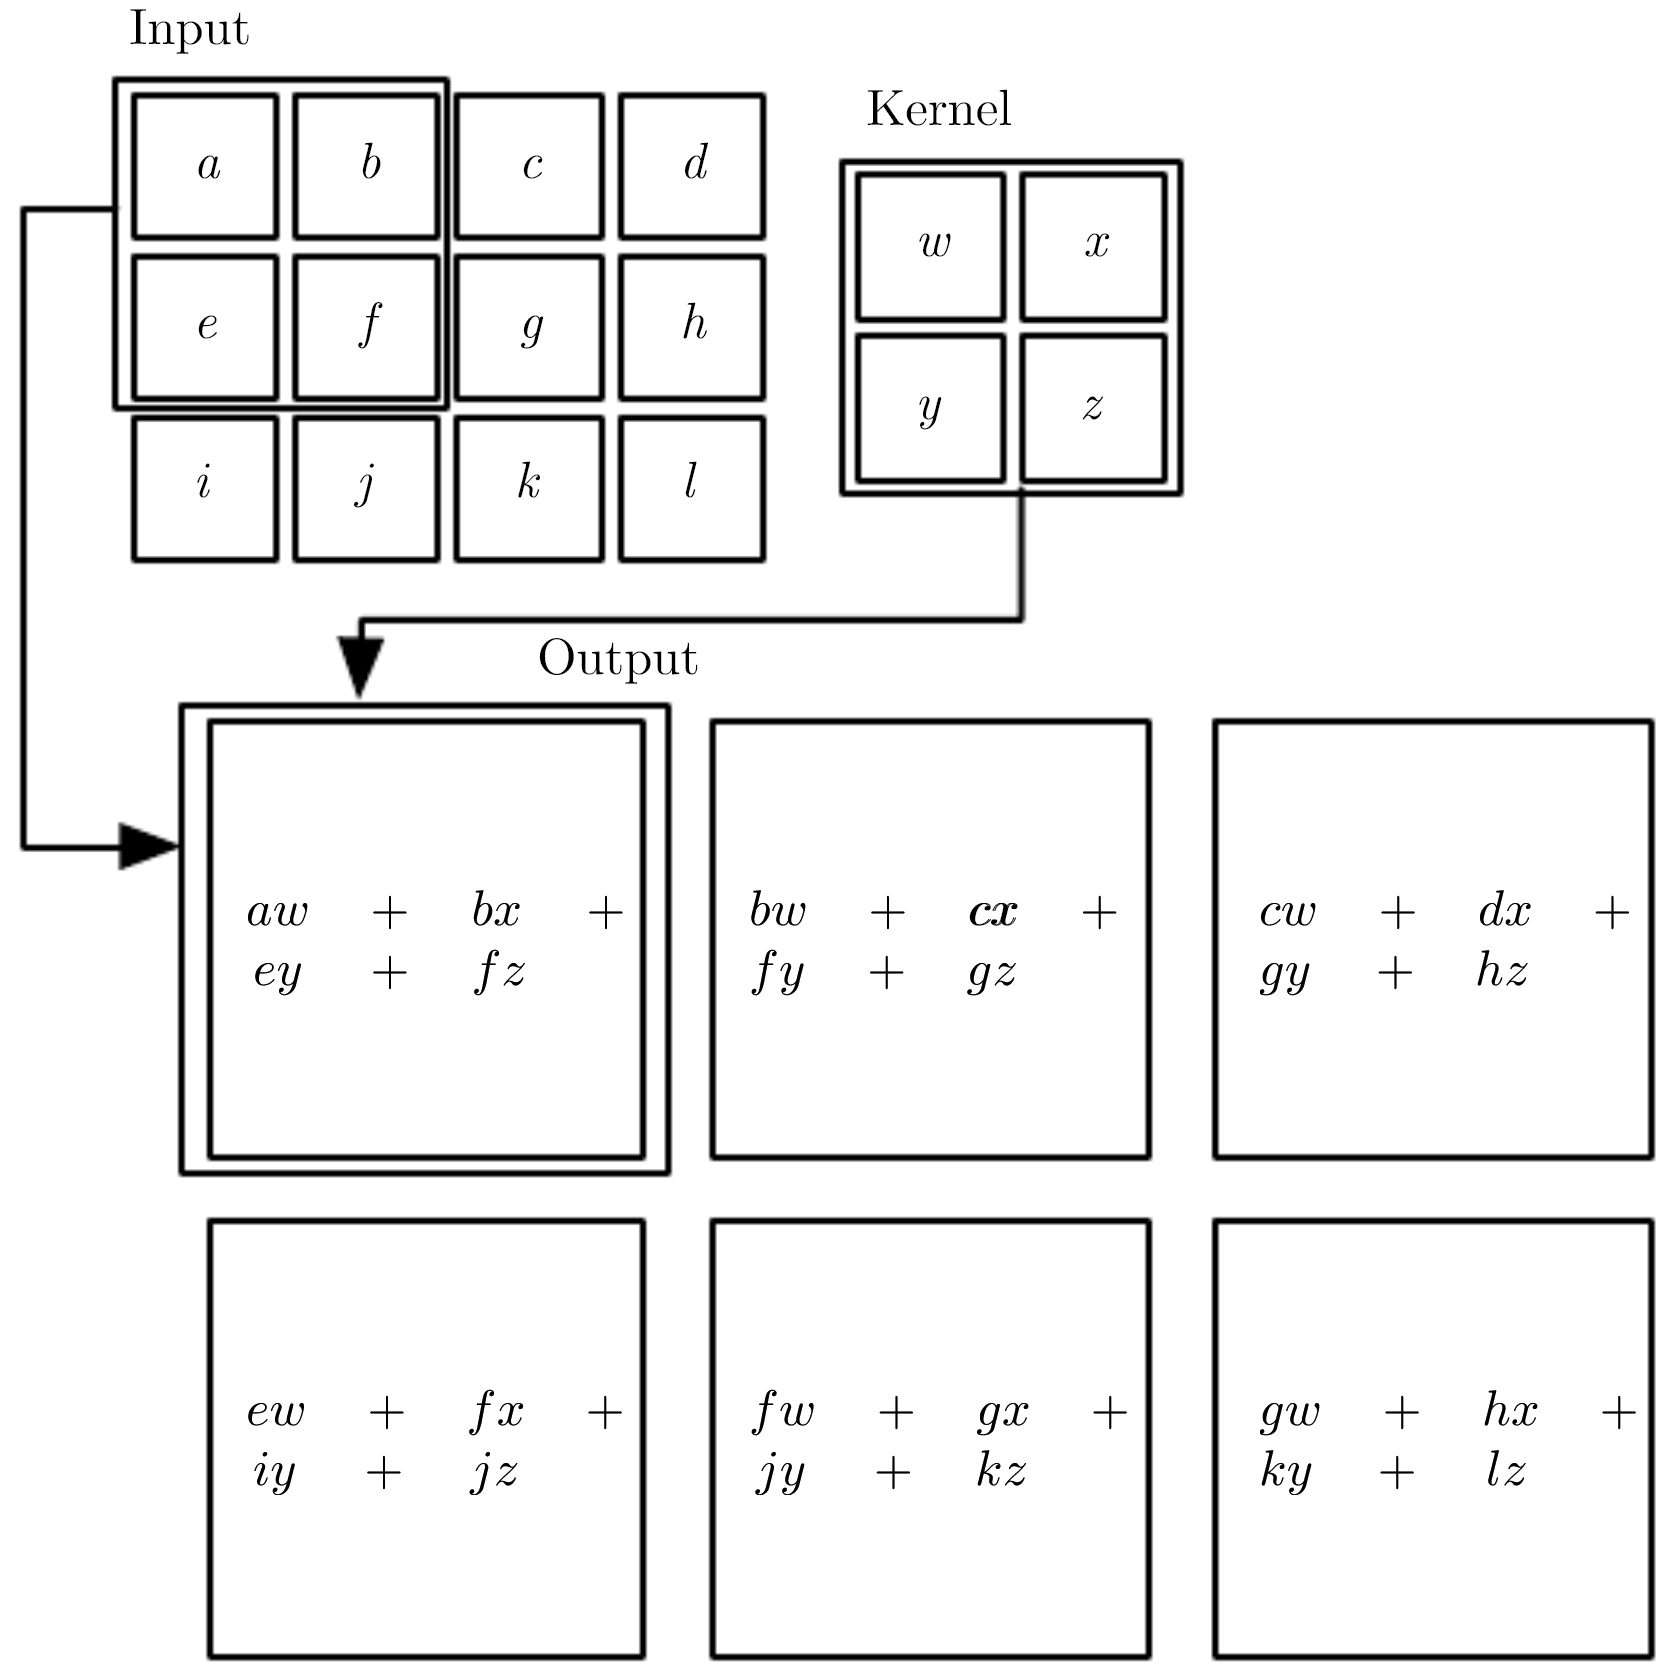
\includegraphics[scale=0.25]{img/convolution.png}
    \caption{An example of a 2-D convolution. (Source: Figure 9.1 from the \citetitle{Goodfellow-et-al-2016} book~\cite{Goodfellow-et-al-2016})}
    \label{fig:conv}
\end{figure}

% RNN
The \textit{recurrent neural network} (RNN) architecture is designed to handle sequential or time series data. RNNs process the sequence one element at a time. The key is that they also maintain a hidden state, or a memory, that captures information about the sequence from element to element. This is achieved by loops in the graph --- the output of an RNN unit (sometimes called a cell) goes back to the same unit as an input with the next element of the sequence (see Figure~\ref{fig:rnn}). Because of the sequential processing, RNNs can process a sequence of an arbitrary length, reusing all the weights for every step. There are multiple options for the basic computational unit that controls how the input is processed and manages the hidden state. We will use the Long short-term memory (LSTM) unit, which is one of the more refined options. RNNs do not have many special hyperparameters. The most important ones include the number of units and the number of layers. There is also the option to make the units bidirectional, which means the sequence is processed both in a forward and a backward direction.

\begin{figure}
    \centering
\begin{tikzpicture}[
    every node/.style={font=\sffamily},
    cell/.style={draw, fill=purple!30, minimum size=9mm, rounded corners},
    arrow/.style={-Stealth, thick},
    input/.style={circle, draw, minimum size=9mm, fill=blue!30, inner sep=0pt},
    output/.style={diamond, aspect=2, draw, minimum size=9mm, fill=green!30, inner sep=0pt},
    skip loop/.style={to path={-- ++(0,#1) -| (\tikztotarget)}},
    hv path/.style={to path={-| (\tikztotarget)}},
    vh path/.style={to path={|- (\tikztotarget)}}
]

% RNN cell before unfolding
\node[cell] (h) {$h$};
\node[input, below=of h] (x) {$x$};
\node[output, above=of h] (o) {$o$};

\draw[arrow] (x) -- node[right] {$U$} (h);
\draw[arrow] (h) -- node[right] {$W$} (o);
\draw[arrow] (h) edge[loop left] node {$V$} (h);

% Unfolding arrow
\draw[arrow, thick, blue] (0.65,0) -- node[above] {Unfold} ++(2.0,0);

% Unfolded RNN cells
\foreach \i in {0,1,2} {
    \node[cell, right=2.5 cm +\i*2 cm of h] (h\i) {$h_{t\ifnum\i>0 +\i\fi}$};
    \node[input, below=of h\i] (x\i) {$x_{t\ifnum\i>0 +\i\fi}$};
    \node[output, above=of h\i] (o\i) {$o_{t\ifnum\i>0 +\i\fi}$};
    \draw[arrow] (x\i) -- node[right] {$U$} (h\i);
    \draw[arrow] (h\i) -- node[right] {$W$} (o\i);
    \ifnum\i>0
        \pgfmathtruncatemacro{\prev}{\i-1}
        \draw[arrow] (h\prev) -- node[above] {$V$} (h\i);
    \fi
}

\draw[arrow] (h2) --node[above] {V} ++(1.5,0);

\end{tikzpicture}

\caption{A single RNN unit. On the left, the RNN unit is compressed and contains a loop connection to itself. On the right, the unit is unfolded, which makes it easier to see how inputs with variable lengths are processed and how the information flows in the network. One of the simplest units could calculate $h_t=\sigma(Vh_{t-1}+Ux_t + b_h)$ and $o_t=\sigma(Wh_{t}+b_o)$.}
\label{fig:rnn}
\end{figure}

% TODO: Transformers

\subsection{Training of neural networks}
% Training of neural networks.
Training of the network can be split into two parts --- the forward pass and the backward pass. These two operations are repeated over and over again until some stopping criterion is met. We call one iteration an epoch. In an epoch, the training algorithm iterates through all examples in the training set, usually grouped in batches. In the forward pass, the network produces an output from the input examples and weights by iteratively going through the graph in a topological order. The loss is calculated from the output of the network and true labels. The gradients of the loss function are computed using the backpropagation algorithm, which iterates through the nodes in reverse order and calculates partial derivatives of the loss with respect to the individual weights.

% Gradient descent algorithm
After the gradients are computed, the loss function is minimized using the gradient descent algorithm. Given a loss function $L(\theta)$ that we want to minimize with respect to the weights, the gradient descent optimizes the function by taking a step in the opposite direction of gradient $\nabla_\theta L(\theta)$, which decreases the loss. That is, the weights are updated using a learning rate hyperparameter $\alpha$: $$ \theta \leftarrow \theta - \alpha \nabla_\theta L(\theta).$$

For this thesis, it is enough to know there is a gradient descent algorithm optimizing the loss and this algorithm and its more advanced derivatives, such as Adam, comes with some hyperparameters. These usually include a \textit{learning rate}, a \textit{momentum}, or a \textit{decay schedule}, if we want to gradually decrease the learning rate. Later, we will also use the fact that training of neural networks is an iterative process, and it usually takes at least tens of epochs until the network starts to converge.

\subsection{Regularization}
% What is regularization
The last concept that is useful to know about for hyperparameter optimization is \textit{regularization}. It is a technique to prevent \textit{overfitting}, which is a situation when the model learns too much from the training set and the validation loss starts increasing because the model learns specific patterns present only in the training dataset. Remember we want the model to generalize well. Regularization is especially important for smaller datasets. There are many regularization techniques and most of them come with some hyperparameter. We call them regularization hyperparameters.

% Examples of regularization
One way to reduce overfitting is to use a \textit{weight decay}, which multiplies the weights by some constant smaller than one and usually close to zero, which we set as a hyperparameter. The intuition behind weight decay is that the network forgets a little each time the weights are updated, so it can learn only general patterns that occur often. Another common regularization technique is the \textit{dropout}. In dropout, some nodes are deactivated during a forward pass with the dropout rate (probability), which is a hyperparameter. The network is forced to work reasonably well with only a subset of nodes, which should also force it to learn general features.


\section{Hyperparameter optimization} \label{sec:hpo}
% Introduction - parameter vs hyperparameter, examples, definitions source
Hyperparameter optimization, or hyperparameter tuning, is the process of selecting the best set of hyperparameters for a machine learning problem. The key distinction between a model parameter and a hyperparameter is that a hyperparameter has to be specified before the training process, while parameters are inferred automatically during the training process. Nevertheless, hyperparameters have a direct influence on the model, as well as the training process. We have already seen hyperparameters related to the training of neural networks, overfitting, underfitting and regularization in the previous section. These hyperparameters alone can make the difference between a model that easily generalizes to unseen examples, and a model that does not predict anything useful. In the following text, we define the hyperparameter optimization problem formally. For that, we use definitions and notation from the paper by \citet{eggensperger2013towards}.

% Define hyperparameters, their impact on model performance, why optimization is important
Let $A$ be a machine learning algorithm with hyperparameters $\lambda_1, \dots , \lambda_n$ with domains $\Lambda_1,\dots , \Lambda_n$. Let $ \mathbf{\Lambda } = \Lambda_1 \times \cdots \times \Lambda_n$ denote its hyperparameter space. Hyperparameters can be continuous, integer-valued, or categorical. There can be conditional hyperparameters, too. We say that hyperparameter $\lambda_i$ is \emph{conditional} on another hyperparameter $\lambda_j$, if $\lambda_i$ is only active if hyperparameter $\lambda_j$ takes values from a given set $V_i(j) \subset \Lambda_j$

For each hyperparameter configuration or setting $\lambda \in \mathbf{\Lambda}$, we denote $A_\lambda$ the learning algorithm A using this hyperparameter setting. Let $\mathcal{L}(A_\Lambda, \: \mathcal{D}_{train}, \: \mathcal{D}_{valid})$ denote the validation loss of algorithm $A_\lambda$ on data $\mathcal{D}_{valid}$ when trained on $\mathcal{D}_{train}$.

\begin{defn}[Hyperparameter optimization problem]\label{defn:x}
The hyperparameter optimization problem is to find hyperparameters $\lambda^*$ that minimize the loss function  \[\lambda^*=\argmin _\lambda f(\lambda)=\argmin_\lambda \mathcal{L}(A_\lambda, \: \mathcal{D}_{train}, \:  \mathcal{D}_{valid}).\]
\end{defn}

Several properties make the problem hard to solve.
\begin{itemize}
    \item It is hard to obtain derivatives of the loss function with respect to hyperparameters and we will not use them to find the optimal solution. Such an optimization problem is called a black-box optimization in literature.
    \item Each function evaluation is expensive. Fully training a single deep neural network can take days.
    \item Each function evaluation may require a variable amount of time. For example, training larger models (e.g. more artificial neurons) takes more time to train. Therefore, the hyperparameter optimization algorithm should take training time into account.
    \item Observations are noisy. Repeated training may result in models that vary in performance since it is common to use random initialization of weights. The training process itself may not be deterministic as well. For example, if we use mini-batch shuffling.
\end{itemize}

On the other hand, we can leverage parallel computation to run multiple trials at the same time. One additional benefit of solving the optimization problem limited to deep neural networks is that we have access to intermediate results, which is not the case for general black-box optimization. This kind of task is sometimes called a grey-box optimization in the literature.

% Note on efficiency

In this thesis, we assume that the general architecture of the neural network is already given and hyperparameters can change only smaller aspects, such as the number of neurons in a layer, or kernel size in a convolutional layer. For literature dealing with the more general problem, please refer to Neural Architecture Search (NAS).

For anyone interested in the process of hyperparameter tuning and how it might be done in practice, we recommend the Deep learning tuning playbook~\cite{tuningplaybookgithub}. The authors give valuable insights into practical aspects of hyperparameter tuning that they have collected over more than ten years of working in deep learning. These insights are rarely documented. As the authors state in the text, they could not find any comprehensive attempt to explain how to get good results with deep learning. More importantly for this thesis, it gives us insight into how experts might do hyperparameter tuning. The text reveals that even today, advanced hyperparameter tuning tools are not the ultimate solution to the problem. Instead, they recommend how to use them smartly. They propose that there is still a human expert guiding the search, at least in the first, exploratory, phase.



\section{Classic Hyperparameter Search Techniques}
% Manual search, grid search, random search
The default approach for many practitioners is manual hyperparameter tuning. We cannot be surprised that people still tune hyperparameters manually. There is no technical overhead or barrier. Also, in the process of hyperparameter tuning, we gain insight into the problem, which might allow us to improve our solution in ways that are not achievable just by hyperparameter tuning. Nevertheless, there are clear limits to manual tuning so let us dive into the algorithmic approaches. The traditional algorithms for hyperparameter optimization are grid search and random search. These algorithms are simple and still widely used.

\paragraph{Grid Search} Grid search performs an exhaustive search through a manually specified subset of the hyperparameter space. Grid search is best used when the number of hyperparameters is small, or the function evaluation is not that expensive. Its biggest drawback is that the number of configurations to evaluate grows exponentially with the number of hyperparameters. Therefore, it is best to determine which hyperparameters are the most important and limit the search only to this subset. If we did not do this, we would waste a lot of computational resources on hyperparameter combinations, where only the unimportant hyperparameter changes, but the important ones stay the same. We illustrate this situation in Figure~\ref{fig:grid}. To mitigate this, we would need a way to determine which hyperparameters are important and need to be tuned together, which is a hard problem itself. On the other hand, grid search is easily parallelizable. That is an enormous advantage since in real-world scenarios, it is not uncommon to have access to a computing cluster.

\paragraph{Random Search} Random search is often used in the HPO literature as the baseline method for more advanced algorithms. In real-world optimization problems, random search often works better than grid search. Bergstra et al.~\cite{bergstra2012random} compared random search to grid search and found that randomly chosen trials are more efficient for hyperparameter optimization than trials on a grid. It is possible to encounter a random search with 2X-budget as a baseline in some research papers. It is just a random search with two times the budget of other methods in comparison. As Li et al.~\cite{li2018hyperband} show, 2X-budget random search provides a strong baseline.

\begin{figure}[H]
    \centering
    \includegraphics[scale=0.8]{img/grid_vs_rs.pdf}
    \caption{A visual comparison of Grid Search versus Random Search. Suppose that we optimize a function with two parameters and the function is the sum of the functions defined for each parameter. The best configuration found after nine trials is highlighted in red. If one of the parameters is not important, grid search wastes resources by repeatedly evaluating similar configurations. }
    \label{fig:grid}
\end{figure}

\paragraph{Quasi-random search} If our budget is low then quasi-random search might be the better option. It works by generating a low-discrepancy sequence. Intuitively, a low-discrepancy sequence covers the whole domain evenly. Therefore, the search space is better covered even with a small number of samples. In the Deep learning tuning playbook, the authors recommend using quasi-random search over grid search and random search for the initial exploration of the hyperparameter space.



\section{Bayesian optimization}
% Going from model-less to model-based approaches
So far, we have seen model-less approaches, where each trial is independent. This approach offers some advantages, like parallelization and simplicity of implementation, but it is quite inefficient. Information obtained from previous trials is not used in any way to guide the search. Bayesian optimization methods build and use an internal model of the learning algorithm's generalization performance. Bayesian optimization is widely covered in literature, we will use the work of Brochu et al.~\cite{brochu2010tutorial} and Frazier~\cite{frazier2018tutorial} for the definitions and the description of the method.

% What is BO and history
% Before mockus was Kushner 1964 and Zilinkas 1975 - 2nd page of Frazier 2018
In general, Bayesian optimization is a class of optimization methods focused on optimizing a real-valued objective function \[ \max_{x\in A} f(x). \] The method got its name from the Bayes' theorem, which is applied by stating that the posterior probability of a model M given observations E is proportional to the likelihood of E given M multiplied by the prior probability of M \[ P(M \given E) \propto P(E \given M)P(M).\] The foundations were laid for Bayesian Optimization by Jonas Mockus~\cite{mockus1974bayesian} in the 1970s and 1980s, but it was not until the early 2000s that Bayesian Optimization got applied to machine learning by Carl Edward Rasmussen~\cite{rasmussen2006gaussian}. Since then, it has become arguably the most prominent advanced technique for hyperparameter optimization, studied by countless groups and being implemented in many popular hyperparameter optimization frameworks.

% BO algorithm introduction
The basic loop of a Bayesian optimization algorithm is simple as shown in Algorithm \ref{alg:bo}. First, the internal model is used to suggest the next hyperparameter configuration to try. This query is much cheaper than evaluating the objective function. We can think of the suggestion as the most promising configuration given the previous observations. More precisely, the algorithm maximizes an \textit{acquisition function} $a$ defined from the \textit{surrogate model}. Then the objective function is evaluated at this configuration and the observed result is added to a database. The surrogate is updated using the database with the new observation and the process is repeated until some stopping condition is triggered, e.g.\ the algorithm runs out of budget.


\begin{algorithm}
    \caption{Bayesian Optimization}
    \begin{algorithmic}[1]
    % \State {\textbf{Initialize}:} Gaussian process prior $GP$, acquisition function $a$, data $\mathcal{D} = \{(x_i, y_i)\}_{i=1}^n$
    \For{$t = 1, \:  2, \ldots $}
        \State Find the next point $x_t$ to evaluate: $x_t = \argmax_{x} a(x \given \mathcal{D}_{1:t-1})$.
        \State Sample the objective function:  $y_t = f(x_t)+ \epsilon_t$.

        \State Augment the data: $\mathcal{D}_{1:t}= \{\mathcal{D}_{1:t-1}, \: (x_t, \: y_t)\}$.
        \State Update the surrogate model given the data $\mathcal{D}_{1:t}$.
    \EndFor
    %\State \textbf{Return} the best point found (e.g., with the lowest $y$)
    \end{algorithmic}
    %\caption{}
    \label{alg:bo}
\end{algorithm}

% Practical considerations - objective function
Before we dive deeper into Bayesian Optimization, let us deal with some practical considerations and properties of the objective function and the feasible set. Since we have defined the hyperparameter optimization problem as minimization of the loss function, we can assume that $f$ is defined as $f(\lambda)=-\mathcal{L}(\lambda)$. Maximizing this function is equivalent to minimizing the original function. We also assume that the objective function is continuous. When we evaluate $f$, we observe only $f(x)$ and no first- or second-order derivatives, which would allow us to use a wider array of optimization methods. We do not know nor assume that $f$ has any special structure like concavity or linearity. To summarize, we can say that Bayesian Optimization is designed for black-box derivative-free global optimization.

% Objective assumptions - Lipschitz-continuous.
% We assume that the objective is Lipschitz-continuous. That is, there exists some constant $C$ such that for all $x_1,x_2\in A: ||f(x_1)-f(x_2)|| \leq C||x_1-x_2||$. The constant $C$ may be unknown.

% Practical considerations - feasible set
We assume further that all inputs $x$ are real-valued, which is not the case for all hyperparameters, and we will address this issue later. Finally, we assume the feasible set $A$ to be a hyper-rectangle $\{ x \in \R \mid a_i \leq x_i \leq b_i \}$, which makes it easy to assess membership.

% Where was Bayesian optimization used?

% General BO Summary
The two main components of a Bayesian Optimization algorithm are a Bayesian statistical model and an acquisition function. The model approximates the objective function including the uncertainty over its predictions and the acquisition function is used for choosing configurations to evaluate. We will go through both of these components in greater detail. First, we will introduce the commonly used acquisition functions, and then we will show three different models.

\subsection{Acquisition functions}
The purpose of an acquisition function is to guide the search. It would be possible to find the predictive mean of the surrogate and sample a configuration that maximizes the mean, but the strength of Bayesian optimization is that it expresses uncertainty. Acquisition functions are designed to take advantage of uncertainty and balance exploration versus exploitation. The acquisition function value might be high if the objective function predicted value is high, but also if the uncertainty of the model is high; the area is not well explored yet but promising. We assume that we have a Bayesian statistical model that for any $x$ in the domain outputs a prediction $y \sim \mathcal{N}(\mu(x), \sigma^2(x))$.

\subsubsection{Upper Confidence Bound}

\begin{figure}
    \centering
    \includegraphics[scale=0.8]{img/ucb_example.pdf}
    \caption{An UCB acquisition function with two $\lambda$ settings demonstrated on a Bayesian model predicting mean $\mu(x)$, and variance (the light blue corresponds to two standard deviations from the mean), fitted to the black true function with four noisy observations.}
    \label{fig:ucb}
\end{figure}

Probably the simplest acquisition function is the Upper Confidence Bound (UCB). Given a mean $\mu(x)$ and a variance $\sigma(x)$, the UCB is calculated as
\[
    \text{UCB}(x) = \mu(x) + \lambda \sigma(x),
\]
where $\lambda$ is an exploration parameter. The smaller the $\lambda$, the more the UCB exploits regions that are known to yield good solutions and vice versa. The UCB acquisition function is illustrated in Figure~\ref{fig:ucb}.

\subsubsection{Probability of Improvement}
Let $y^*=\max_{i\in[1..n]} f(x_i)$ be the value of the best point evaluated so far after $n$ iterations and let $x$ be the next point we consider sampling. We define an improvement random variable as
\[
    I(x) \coloneq \max(f(x) - y^*,0).
\]

The probability of improvement acquisition function assigns to each candidate $x$ the probability of $I(x) > 0$. We can write
\[
    PI(x) = P(I(x) > 0) = P(f(x) > y^*) = 1-P(f(x) \leq y^*).
\]
Since we assume that $f(x)$ is normally distributed, then the PI is calculated from the cumulative density function $\Phi$ of normal distribution. We remind that for $X \sim \mathcal{N}(\mu,\sigma^2)$, we calculate $P(X \leq x)$ as $\Phi ((x-\mu)/\sigma )$. We also use the property $1-\Phi(x)=\Phi(-x)$. Therefore, the PI is calculated as follows:

\[
    PI(x) = 1 - \Phi\left(\frac{y^*-\mu(x)}{\sigma(x)}\right) = \Phi\left(\frac{\mu(x)-y^*}{\sigma(x)}\right).
\]

The problem with PI is that it does not factor in the magnitude of improvement. In the standard form, PI cares only about being as certain as possible about improving upon the current best solution. This often results in PI suggesting points close to the optimum, i.e.\ PI is biased towards exploitation. This problem is alleviated by adding a new parameter $\xi$, which forces PI to consider only points that are by at least $\xi$ better than the current best solution:
\[
    PI(x)=P(I(x)>\xi)
\]

\subsubsection{Expected improvement}
Expected improvement (EI)~\cite{jones1998efficient} enhances PI by considering the magnitude of improvement as well as the probability of improvement. That is achieved by taking the expected value of $I(x)$. Using the assumption that $I(x)$ is normally distributed, the density of $I(x)$ for a specific value of improvement, $I$, is given by
\[
\frac{1}{\sqrt{2 \pi}\sigma(x)} \text{exp}\left(-\frac{(\mu(x)-y^*-I)^2}{2\sigma^2(x)}\right).
\]
% TODO: Is the random variable notation used correctly here for $I(x)$? Is it a problem that we cut off the improvement at 0? Probably Okay

The expected value is calculated by integrating the density function multiplied by the improvement:
\[ EI(x) = \mathbb{E}[I(x)] = \int_{I=0}^{I=\infty} I\frac{1}{\sqrt{2 \pi}\sigma(x)} exp\left(-\frac{(\mu(x)-y^*-I)^2}{2\sigma^2(x)}\right) dI. \]
The analytical solution to this integral can be found in the literature~\cite{jones1998efficient} and it is as follows:
\[ EI(x) = (\mu(x)-y^*)\Phi(Z)+\sigma(x)\phi(Z), \]
where
\[ Z=\frac{\mu(x)-y^*}{\sigma(x),} \]
and $\phi$ is the density of the normal distribution.

Even the expected improvement can be extended with parameter $\xi$ as in the PI acquisition function. The role of this parameter stays the same; it enables us to balance exploration and exploitation. The modified acquisition function is
\[
EI(x) = (\mu(x)-y^*-\xi)\Phi(Z)+\sigma(x)\phi(Z), \]
where
\[ Z=\frac{\mu(x)-y^*-\xi}{\sigma(x)}. \]
 Expected improvement is a popular acquisition function that balances the exploration-exploitation trade-off well; it prioritizes exploring regions with a high probability of significantly improving upon the current best solution. We compare all the mentioned acquisition functions in Figure~\ref{fig:ei}.

 \begin{figure}
    \centering
    \includegraphics[scale=0.8]{img/acq_example.pdf}
    \caption{A comparison of different acquisition functions. The top image shows the real target function with a Bayesian model predicting mean and variance (the light blue area corresponds to two standard deviations). The other images show different acquisition functions from top to bottom: upper confidence bound, probability of improvement, and expected improvement.}
    \label{fig:ei}
\end{figure}

% TODO: Include other acquisitions if needed, like entropy search, or knowledge gradient
% PI is for maximization
%Probability of improvement~\cite{kushner1964new} \[ \text{PI}(x) = P(y > y^* \given x) = \int_{y^*}^{\infty} p(y \given x) \, dy \]

%Entropy search
%Knowledge gradient

\newpage
\subsection{Gaussian Process Regression}
% Why is Gaussian process regression the default choice for Bayesian Optimization
The standard model in the Bayesian Optimization literature is the Gaussian Process (GP) regression. An intuitive introduction to the topic was published by \citet{wang2023intuitive}. Because the presentation of the topic is clear and concise in Wang's work, we have rewritten and adapted this approach in our own words. The definitions and the notation are taken from the textbook by Rasmussen~\cite{rasmussen2006gaussian}. There are many other machine learning algorithms for regression, but Gaussian processes offer a unique mix of properties that make them the natural choice. One of the most important properties of GPs is that they quantify the uncertainty, which allows us to incorporate it into our sampling strategy --- the areas with the most uncertainty should likely be explored more, or similar heuristic strategy. Another advantage is the possibility of incorporating our prior beliefs about the objective function with the kernel function. As a result, Gaussian processes are remarkably efficient when the amount of data is limited. On the other hand, GPs do not scale well with large datasets, because of their $\mathcal{O}(n^3)$ complexity. In practice, GPs limit us to the number of samples in the order of hundreds.

\subsubsection{Gaussian distribution}
% Univariate normal distribution
In order to describe the Gaussian process regression, we will start with the basics. A random variable X is Gaussian or normally distributed with mean $\mu$ and variance $\sigma^2$ if its probability density function is: \[ P_X(x) = \frac{1}{\sqrt{2\pi} \sigma} \exp\left(-\frac{(x-\mu)^2}{2 \sigma^2}\right). \] We denote that a random variable is normally distributed as $X \sim \mathcal{N}(\mu, \sigma^2)$. For illustration, we have sampled 500 points randomly from a univariate normal distribution into a vector $x_1 =[x_1^1,x_1^2, \ldots,x_1^{500}]$. In Figure~\ref{fig:1} we plot a histogram of the points and fit a Gaussian distribution over them. We also plot the points vertically along the Y-axis, which is the first step towards the Gaussian process regression.

\begin{figure}
    \centering
    \begin{subfigure}{0.49\textwidth}
        \centering
        \includegraphics[scale=0.8]{img/1d_gaussian.pdf}
        \caption{Histogram of the samples with the fitted density as a black curve.}
%        \label{fig:f1}
    \end{subfigure}
    \hfill
    \begin{subfigure}{0.49\textwidth}
        \centering
        \includegraphics[scale=0.8]{img/1d_gaussian_projected.pdf}
        \caption{Random samples plotted vertically along the Y-axis with a fixed X coordinate.}
 %       \label{fig:f2}
    \end{subfigure}
    \caption{A visualization of sampling from a Gaussian distribution. A random variable $X \sim \mathcal{N}(0, 1)$ is sampled 500 times.}
    \label{fig:1}
\end{figure}

% Connecting several univariate Gaussian distributions
Similarly, we could sample several vectors $x_1,\ldots,x_n$ of points and plot them with a different x-coordinate as shown in Figure~\ref{fig:2}. If we connect the corresponding samples with a line, we could perform a regression task using these lines in the domain $[0,1]$. The issue is that the samples generating the lines are independent, making the predictions of no use. The key assumption for regression is that close points have similar values. Therefore, we have to find a way to introduce a correlation between the samples, preferably based on their distance.

% Connected distributions
\begin{figure}
    \centering
    \begin{subfigure}{0.49\textwidth}
        \centering
        \includegraphics[scale=0.8]{img/10_gaussians.pdf}
        \caption{Random samples}
%        \label{fig:f1}
    \end{subfigure}
    \hfill
    \begin{subfigure}{0.49\textwidth}
        \centering
        \includegraphics[scale=0.8]{img/10_gaussians_conn.pdf}
        \caption{Random samples connected by linear lines}
 %       \label{fig:f2}
    \end{subfigure}
    \caption{N=5 sampled random vectors, each with M=10 random samples drawn from a normal distribution. Samples from each vector are plotted along the Y-axis with the same X coordinate}
    \label{fig:2}
\end{figure}

% Multivariate normal distribution
A set of correlated, normally distributed random variables is described by the \textit{multivariate normal distribution} (MVN). We denote MVN as $\mathbf{X} \sim \mathcal{N}_k(\mathbf{\mu}, \mathbf{\Sigma})$, where $\mathbf{X}=(X_1,X_2,\ldots ,X_n)^T$ is a random vector, $\mathbf{\mu}= (\mu_1,\mu_2,\ldots , \mu_n)^T$ are the means and $\mathbf{\Sigma} \in  \R^{k \times k}$ is the covariance matrix. The $k$ is often omitted as the dimensions are usually clear from the context. The covariance matrix specifies the covariance between each pair of elements of a given random vector, with $\Sigma_{ij} = \text{cov}[X_i, X_j]$. The $\mathbf{\Sigma}$ is a symmetric and positive semi-definite matrix with variances on its main diagonal. Finally, the probability density function of k-dimensional MVN is defined as \[ \mathcal{N}(\mathbf{x} \given \mathbf{\mu}, \mathbf{\Sigma}) = \frac{1}{(2\pi)^{k/2} |\mathbf{\Sigma}|^{1/2}} \exp \left(-\frac{1}{2} (\mathbf{x} - \mathbf{\mu})^T \mathbf{\Sigma}^{-1} (\mathbf{x} - \mathbf{\mu}) \right). \]

% Bi-variate example

% Conditional MVN is also MVN
For regression, we are more interested in conditional probability rather than joint probability, as we want to make use of the observed data points. To get the conditional probability, we can partition the random vector $\mathbf{X}$ into $\mathbf{X_1}$ and $\mathbf{X_2}$. The conditional probability of $\mathbf{X_1}$ given $\mathbf{X_2}$ is also an MVN because a multivariate normal distribution is closed under conditioning. We will show the exact formulas in the description of Gaussian process regression.

%
\subsubsection{Kernels}
% Kernels in general - smoothens the functions
Using the multivariate normal distribution, we can correlate the points of our regression function. Instead of manually specifying the covariance matrix, we will use kernels. A kernel function measures the similarity between a pair of data points. This in turn impacts the smoothness of the regression functions --- we want close points to have similar function values, and we use the kernel function to determine the strength of the correlation.

% RBF kernel, Figure with samples with RBF covariance
A common choice is the squared exponential kernel, also called the Radial Basis Function (RBF) kernel, defined as \[ K(x, x') = exp \left( -  \frac{||x - x'||^2} {2 \sigma^2}\right). \] The kernel has a parameter $\sigma$ called the length scale. It controls how quickly the correlation between two points decays. The functions predicted by the kernel are smooth and infinitely differentiable. We have plotted samples of the twenty-variate normal distribution with RBF kernel as covariance function in Figure~\ref{fig:f3}. Note that the samples illustrated in Figure~\ref{fig:2} can also be viewed as being drawn from MVN distribution, but with an identity covariance function, which highlights the role of a kernel.

% Lines drawn using samples from Multivariate normal distribution
\begin{figure}
    \centering
    \includegraphics[scale=0.8]{img/20_gaussians_with_prior.pdf}
    \caption{Samples from the 20-VN distribution with RBF covariance.}
    \label{fig:f3}
\end{figure}
% For two separate figures, I would use minipage

% The 'kernel trick'

% Infinite dim MVN
We have now covered all the background necessary to get to Gaussian processes. We understand how the MVN is used with kernels to produce correlated predictions that look smoother when connected with lines. As we increase the dimensions of the MVN, the points will get closer and closer together in the domain of interest. For a truly smooth prediction spanning the whole domain, we use MVN distribution with infinite dimensions. % We call such functions \textit{kernelized prior functions}.


\subsubsection{Gaussian processes}
% Parametric vs non-parametric models
%Gaussian processes are a non-parametric model, meaning that there are no parameters that define the regression function such as $\theta_1$ and $\theta_2$ in a linear regression model $y = \theta_1 + \theta_2 x$. After a parametric model is trained, the predictions no longer depend on the training data and all the information is encapsulated in the parameters. Instead, non-parametric models do not assume any specific form for the relationship between independent and dependent variables and the model structure is determined by the data itself.

\begin{figure}
    \centering
    \includegraphics[scale=0.8]{img/gaussian_process.pdf}
    \caption{An example of Gaussian process regression. The black dashed line is the true target function. We drew six random samples and the function was evaluated at these points with noise (blue crosses). Then we sampled 15 functions from the posterior distribution given the test points. The blue line is the mean function and the light blue area is bounded at two standard deviations from the mean.}
    \label{fig:f4}
\end{figure}

% Introduction (infinite MVN), example
Gaussian processes are a generalization of MVN into infinite dimensions. The kernel specifies permissible functions which make up the prior distribution. The Gaussian process model defines a probability distribution over prior functions that fit the observed data. The concept is best illustrated in an example. In Figure~\ref{fig:f4}, we want to perform a regression task over the true (black) function. We are given six noisy observations. We can derive the (blue) mean function by calculating the posterior distribution and averaging over all functions weighted by their posterior probability. For the illustration of the posterior distribution, we can observe the light blue area marking two standard deviations from the mean. Lastly, the colorful functions are randomly sampled from the posterior distribution.

Let us define the Gaussian process formally. Let $\mathbf{X}=[\mathbf{x_1}, \ldots ,\mathbf{x_n}]$ represent the observed data points, $\mathbf{f}=[f(\mathbf{x_1}), \ldots ,f(\mathbf{x_n})]$ the function values, $\mathbf{\mu}=[m(\mathbf{x_1}),\ldots , m(\mathbf{x_n})]$ the mean function, and $K_{ij}=k(\mathbf{x_i}, \mathbf{x_j})$ the positive definite kernel function. The mean function represents a prior mean --- our initial belief about the average behavior of the function across the input space --- and is often just assumed to be $0$. Let us consider a regression task. We want to predict function values $\mathbf{f}(\mathbf{X}_*)$ at new points $\mathbf{X}_*$ using the Gaussian process regression. The joint distribution of $\mathbf{f}$ and $\mathbf{f_*}$ is given by
\[
\begin{bmatrix}
    \mathbf{f} \\ \mathbf{f}_*
    \end{bmatrix}
    \sim
    \mathcal{N} \left(
    \begin{bmatrix}
    m(\mathbf{X}) \\ m(\mathbf{X}_*)
    \end{bmatrix} ,
    \begin{bmatrix}
    \mathbf{K} & \mathbf{K}_* \\
    \mathbf{K}_*^T & \mathbf{K}_{**}
    \end{bmatrix}
    \right) \ ,
\]
where $\mathbf{K}=K(\mathbf{X},\mathbf{X})$, $\mathbf{K}_*=K(\mathbf{X},\mathbf{X}_*)$, $\mathbf{K}_{**}=K(\mathbf{X}_*,\mathbf{X}_*)$, and we assume that $(m(\mathbf{X}),m(\mathbf{X_*}))=\mathbf{0}$.

Since we solve the regression task, we are interested in the conditional distribution $P(\mathbf{f}_* \given \mathbf{f},\mathbf{X}, \mathbf{X_*})$, not the joint distribution. Using the formula for MVN conditional distribution, it can be derived from the joint distribution $P(\mathbf{f}_*,\mathbf{f} \given \mathbf{X}, \mathbf{X_*})$ as
\[ \mathbf{f}_*  \given  \mathbf{f}, \mathbf{X}, \mathbf{X_*} \sim \mathcal{N} \left(
    \mathbf{K}^T_* \mathbf{K}^{-1} \mathbf{f}, \ \mathbf{K}_{**} - \mathbf{K}^T_* \mathbf{K}^{-1} \mathbf{K}_*
 \right) \ .
 \]

 We often encounter noisy observations in practice, which is often the case for the hyperparameter optimization problem as well. We deal with noisy observations by assuming additive independent and identically distributed Gaussian noise $\epsilon$ with variance $\sigma_n^2$. The noise is incorporated into the prior as $\text{cov}(y)= \mathbf{K}+\sigma_n^2 \mathbf{I}$. Then the observations can be expressed as $y=f(\mathbf{x})+ \epsilon$. The joint distribution with noise is
 \[
\begin{bmatrix}
    \mathbf{y} \\ \mathbf{f}_*
    \end{bmatrix}
    \sim
    \mathcal{N} \left(
    \mathbf{0},
    \begin{bmatrix}
    \mathbf{K} + \sigma^2_n \mathbf{I} & \mathbf{K}_* \\
    \mathbf{K}_*^T & \mathbf{K}_{**}
    \end{bmatrix}
    \right) \ .
\]

Finally, the conditional distribution with noise is derived as
\[ \mathbf{\bar{f}}_* \given \mathbf{y}, \mathbf{X}, \mathbf{X_*} \sim \mathcal{N} \left(
    \mathbf{\bar{f}_*}, \text{cov}(\mathbf{f_*})
 \right) \ ,\]
 where

  \begin{align*}
  \mathbf{\bar{f}}_* &\overset{\Delta}{=} \mathbb{E}[ \mathbf{\bar{f}}_*  \given  \mathbf{y}, \mathbf{X}, \mathbf{X}_*] \\
                    &= \mathbf{K}^T_*[\mathbf{Κ} + \sigma^2_n \mathbf{I}]^{-1} \mathbf{y}\ \text{,} \\
          \text{cov}(\mathbf{f}_*)  &= \mathbf{K}_{**} - \mathbf{K}_*^T[\mathbf{K}+\sigma^2_n\mathbf{I}]^{-1}\mathbf{K}_* \ \text{.}
  \end{align*}

% Include the algorithm 2.1. from Rasmussen?


% General recommendations when to use GPR
Gaussian processes are best suited for optimization over continuous domains of less than 20 dimensions and when the number of function evaluations is very low. GPs tolerate stochastic noise in function evaluations~\cite{frazier2018tutorial}.

% "For continuous functions, Bayesian optimization typically works by assuming the unknown function was sampled from a Gaussian process and maintains a posterior distribution for this function as observations are made or, in our case, as the results of running learning algorithm experiments with different hyperparameters are observed (Practical Bayesian optimization 2012)"


% Good overview of Gaussian processes: \cite{brochu2010tutorial}.

% Practical BO of ML algorithms. They show how different kernels affect performance and describe algorithms that take into account the variable cost (duration) of learning algorithm experiments~\cite{snoek2012practical}.


\subsection{Tree-Structured Parzen Estimator}

Another popular Bayesian optimization method for hyperparameter optimization is the Tree-structured Parzen Estimator (TPE) introduced by~\citet{bergstra2011algorithms}. As the name suggests, it is an extension of a Parzen estimator to a tree-structured search space. Therefore, TPE can handle conditional parameters as well, which is one of its advantages over GPs. A Parzen estimator, also known as a kernel density estimator (KDE), is a non-parametric method used to estimate the probability density function of a random variable based on a set of observed data points. Instead of assuming the underlying distribution and fitting it to the data, a Parzen estimator uses a kernel function to determine the shape and influence of each data point on the estimated probability density function. We provide a brief explanation of the inner workings of TPE, primarily based on the work of \citet{watanabe2023tree}.

In the TPE algorithm, two kernel density estimators are used. Keeping the notation from the original paper~\cite{bergstra2011algorithms}, we want to minimize the objective function $f(x)$ and the observations $\mathcal{D}$ are split into the better (lower) group $\mathcal{D}^{(l)}$ and the worse (greater) group $\mathcal{D}^{(g)}$ based on their objective value; for illustration see the top left part of Figure~\ref{fig:tpe}. More precisely, the top-quantile $\gamma$ is computed in each iteration based on the number of observations $N=|\mathcal{D}|$ and $y^{\gamma}$ is the top-$\gamma$-quantile objective value in the set of observations $\mathcal{D}$. Observations with $y\leq y^\gamma$ are assigned into the $\mathcal{D}^{(l)}$, and observations with $y > y^\gamma$ to the $\mathcal{D}^{(g)}$. The subsets are used to model $p(\mathbf{x} \given y, \mathcal{D})$ with the assumption:
\begin{equation} (\mathbf{x} \given y, \mathcal{D})\coloneq  \left\{
  \begin{array}{ll}
        p(\mathbf{x} \given \mathcal{D}^{(l)}) \quad  &(y \leq y^\gamma) \\
        p(\mathbf{x} \given \mathcal{D}^{(g)}) \quad  &(y > y^\gamma)
  \end{array}
  \right. .
  \label{eqn:tpe:assumption}
\end{equation}

\begin{figure}
    \centering
    \includegraphics[scale=0.40]{img/tpe-conceptual.pdf}
    \caption{Example of the TPE algorithm. We are searching for the minimum of the target (black) function. The observations are split into $D^{(l)}$ and $D^{(g)}$ by the green line on the objective value of observations. For each group, a kernel density estimation is calculated. The acquisition function is derived from the densities and the algorithm chooses the next point to sample by finding the maximum (Source: Figure 1 from Watanabe~\cite{watanabe2023tree}).}
    \label{fig:tpe}
\end{figure}

Now we can show how the kernel density estimations from the equation above are calculated. Let us assume the $D$ is sorted by $y_n$ such that $y_1 \leq y_2 \leq \cdots \leq y_N$. Then the KDEs are estimated as


\begin{equation}
    \begin{split}
   p(\mathbf{x} \given \mathcal{D}^{(l)}) &= w_0^{(l)} p_0(\mathbf{x}) + \sum_{n=1}^{N^{(l)}}w_n k(\mathbf{x},\mathbf{x}_n \given b^{(l)}), \\
   p(\mathbf{x} \given \mathcal{D}^{(g)}) &= w_0^{(g)} p_0(\mathbf{x}) + \sum_{n=N^{(l)}+1}^{N}w_n k(\mathbf{x},\mathbf{x}_n \given b^{(g)}),
    \end{split}
    \label{eqn:tpe:kdes}
\end{equation}

\noindent
where $k$ is a kernel function, the weights $\{ w_n \}_{n=1}^N$ are recomputed every iteration, $b^{(l)},b^{(g)} \in \R_+$ are the bandwidth and $p_0$ is non-informative prior. The KDEs are illustrated in the top right part of Figure~\ref{fig:tpe}.

The last part of the algorithm yet to be described is the acquisition function. It is calculated from the KDEs using the assumption from Eq.~\ref{eqn:tpe:assumption} as
\[
\mathbb{P}(y \leq y^\gamma \given \mathbf{x},\mathcal{D}) \overset{\text{rank}}{\simeq} r(\mathbf{x} \given \mathcal{D}) \coloneq  \frac{p(\mathbf{x} \given \mathcal{D}^{(l)})}{p(\mathbf{x} \given \mathcal{D}^{(g)})} ,
\]
where the $\overset{\text{rank}}{\simeq}$ symbol means the order isomorphic between the left-hand side and the right-hand side. See Figure~\ref{fig:tpe} for illustration. The detailed pseudocode is provided in Algorithm~\ref{tpe-algo}.
% TODO: Why use TPE instead of GP?

\subfile{./alg/tpe-algo.tex}

% \subsubsection{Components and control parameters}
% \xxx{In this section, we will look at how the different components and control parameters change the behavior of the algorithm}. We start with the \emph{splitting algorithm}, which is used to split the observations $\D$ into $\Dl$ and $\Dg$. Weighting Algorithm. Kernel Functions (numerical, categorical, univariate vs multivariate). Bandwidth. Non-informative prior. \xxx{Will I have to go into such a details?}

\subsection{Random Forest}
The last Bayesian optimization surrogate that we are going to introduce is the random forest model. This approach was first introduced by Hutter et al.~\cite{hutter2010sequential} as SMAC, which stands for Sequential Model-based Algorithm Configuration. It was published as an alternative to the Gaussian processes for the general algorithm configuration problem, approximately at the same time as the TPE.\@ The random forest surrogate is still widely used, mostly in the updated SMAC3 Python package~\cite{smac3}.

Random forest~\cite{breiman2001random} is a machine learning method for classification and regression that trains an ensemble of decision trees and predicts the combined value from all the decision trees during inference. In SMAC, random forests are used for regression to directly model the objective function. The advantage of using regression trees is that they perform well on categorical input data, unlike Gaussian processes. The model is trained by randomly sampling $n$ data points with repetition for each of $B$ regression trees. At each split point in a tree, only a random subset of features is considered. The default is $5/6$ of all features. The default number of regression trees in the algorithm $B$ is set to $10$. There is one more parameter $n_{min}$ for the minimal number of data points required to split a node. This parameter is set to $n_{min}=10$ by default.

Prediction for a new data point is the empirical mean of individual trees' predictions. A prediction of a single tree is usually the mean of the data points in the leaf that corresponds to the input configuration, but the authors implement an option for a user-defined prediction function as well. The algorithm also calculates the empirical variance from the predictions of the individual trees. To select the next configuration to evaluate, the expected improvement acquisition function is maximized. SMAC solves the maximization problem by a multi-start local search. According to the authors, this method provides better results than random sampling.
% Could write a little more about the local search.

\chapter{Multi-fidelity optimization}
% TODO: Multi-fidelity = gray-box optimization
% TODO: Maybe do an overview of the methods and approaches here first

% Introduction - more efficiency by getting early estimates
Even though Bayesian optimization techniques are more sample-efficient compared to a random search, there is another family of approaches that strive to improve the search efficiency further. Instead of training the network until full convergence to obtain the performance metric, multi-fidelity techniques make use of the assumption that a good enough approximation of the final performance can be obtained much faster --- either by stopping early or by training the model on a subset of the training data. This either reduces the computation time or allows the algorithm to evaluate more configurations in the same amount of time. The actual efficiency gain depends on the quality of the intermediate results. The training of neural networks is an inherently noisy process, which makes the problem more challenging. Nevertheless, many approaches successfully exploit multi-fidelity evaluations.

% Fidelity hyperparameter, relationship fidelity vs reliability, rank correlation
Formally, a new hyperparameter $\lambda_{fid}\in [0,1]$ is introduced that allows us to evaluate the function $f(x, \lambda_{fid})$ using just a $\lambda_{fid}$ portion of the full budget (e.g.\ epochs). In most of the literature, the term \textit{budget} is used for specifying the fidelity. Determining the fidelity at which to evaluate the function is the challenging task. Usually, the algorithm has no prior knowledge of the relationship between different fidelities, as well as the reliability of the estimates. That is why most of the multi-fidelity algorithms use some kind of schedule to progressively increase the fidelity hyperparameter.

% Often the algorithms do not try to predict the final performance from low-fidelity evaluations at all. They just compare several configurations at the same fidelity level, hoping the ranking will be similar at a higher fidelity. If a low-fidelity ranking predicts a high-fidelity ranking well, we say that the rank correlation is high. In practice, the reliability of estimates and rank correlation usually gets better as the $\lambda_{fid}$ is increased.

% Don't use multi-fidelity for everything - transfer learning
Finally, we should also note that multi-fidelity techniques are not the universal solution to every hyperparameter optimization problem. If the optimization budget is high, standard random search or Bayesian optimization might perform better, because the partial evaluations can be misleading and good configurations might be discarded too soon. Multi-fidelity techniques usually provide the greatest benefits on a low budget. Often some information is already known before the tuning process. It could be an experience with the same model, or with a similar dataset, that gives us an idea of which hyperparameter configuration might perform well. We might even have logs of a previous hyperparameter tuning experiment that is similar to the current task. In that case, there is a subfield of hyperparameter optimization called \textit{transfer learning} that deals with the problem of reusing previous experience to speed up the search. Transfer learning methods range from simply suggesting a few configurations that we think could perform well to sophisticated pre-trained Gaussian processes and kernels. Transfer learning methods are beyond the scope of this thesis, and we refer the reader to the literature~\cite{bardenet2013collaborative, yogatama2014efficient,perrone2018scalable} for further details.


% Collaborative hyperparameter tuning~\cite{bardenet2013collaborative}.
% Efficient transfer learning method for automatic hyperparameter tuning~\cite{yogatama2014efficient}.
%Scalable hyperparameter transfer learning~\cite{perrone2018scalable}.
%Pre-trained Gaussian processes for Bayesian optimization~\cite{wang2021pre}.

\section{Early stopping}

\subsection{Learning curve extrapolation}
% Freeze-thaw paper - extrapolating of learning curves with new kernel (infinite mixture of exponentially decaying basis functions - TODO), Bayesian optimization,
% Authors state there is possible extension to more flexible priors such as spatio-temporal GP with separable covariance
The simplest way to reduce the runtime of an algorithm is to stop the computation before it finishes. Swersky et al.~\cite{swersky2014freeze} noticed that human experts have the ability to assess whether the model will eventually be useful early in the training and developed a method to leverage early stopping. They refer to this method as freeze-thaw Bayesian optimization, because it allows for pausing or aborting the training procedure when the model does not seem promising and resuming the training later if needed. This is combined with the Bayesian optimization framework for hyperparameter search and the authors propose a technique for estimating when to pause and resume training. The algorithm uses an information-theoretic criterion to determine which models to thaw.

% More freeze-thaw and Domhan interpolation of learning curves
Freeze-thaw method relies on the assumption that for many models the training loss roughly follows an exponential decay. Swersky et al.~\cite{swersky2014freeze} developed a new kernel to serve as a prior characterizing the learning curves. This kernel is then used to forecast the final training loss and to provide these estimates to the Bayesian optimization. The kernel was successfully applied to matrix factorization and other problems, but it did not describe the learning curves of deep neural networks well. The same idea was explored by Domhan et al.~\cite{domhan2015speeding}, but with a focus on deep neural networks. They developed a probabilistic model to extrapolate learning curves and used it to terminate training runs likely to perform worse than the best model so far. The authors modeled learning curves as a combination of eleven different model families because they concluded that even though all of these models capture certain aspects of learning curves, no single model can describe all learning curves by itself. Their approach is agnostic to the hyperparameter optimizer and sped up the hyperparameter optimization approximately by a factor of two. Even though the extrapolation of learning curves is a promising approach, it did not catch up.

\subsection{Successive Halving}
% Successive Halving is widespread
 Arguably the most influential approach to multi-fidelity optimization is the Successive Halving algorithm proposed by Jameison and Talwalkar~\cite{jamieson16}. Even though the algorithm is rarely used in its original form, the success of Successive Halving stems from the fact that the algorithm has been used as a basis by many other researchers, presumably for its simplicity and robustness. Successive Halving solves the problem of efficient budget allocation by iteratively increasing the fidelity only for the best candidates. Note that both fidelity and budget denote the same resource in this case.

 % How it works
 The algorithm works in rounds, each round has the same fixed budget $B$ that is uniformly distributed between the candidate solutions. First, it starts with $n$ randomly sampled configurations and the budget is set as $B \leftarrow nb_0$, where $b_0$ is the minimal budget. For simplicity, we can assume that $b_0=1$, which means that in the first round, the budget $B=n$ is uniformly distributed between the $n$ solutions, so each candidate solution is trained for one epoch. After the intermediate results are obtained for all solutions, the algorithm discards the worst half and the first round ends. Since only half of the solutions are left now and the budget for each round is fixed, each solution is allocated twice the budget in the next round. This process is repeated until a single configuration remains. The pseudocode of the generalized algorithm is provided in the Algorithm~\ref{alg:sh}. The only difference is that the generalized algorithm uses a \textit{reduction factor} $\eta$ --- it keeps only $1/\eta$ of the best configurations and the budget is increased by the factor of $\eta$.

 \begin{algorithm}
    \caption{Successive Halving}
    \begin{algorithmic}[1]
    \Statex {\textbf{Input}:} Search space $\mathcal{X}$,\hspace{1mm} number of initial configurations $n$ ,\hspace{1mm} min budget $b_0$,\hspace{1mm} max budget $B$,\hspace{1mm} reduction factor $\eta$.
    \State{$b \leftarrow b_0$}
    \State{Sample $n$ configurations $X \subset \mathcal{X}$ at random.}
    \While{$b \leq B $}
        \For{$x \in X$}
            \State Evaluate x for a budget of b.
        \EndFor
        \State $b \leftarrow \eta b$
        \State Select the $1/\eta$ best performing configurations in $X$ and discard the rest.
    \EndWhile
    \end{algorithmic}
    \label{alg:sh}
\end{algorithm}

% Example computation to illustrate efficiency
To illustrate the efficiency of the algorithm, let us consider a practical example. Suppose we want to optimize the hyperparameters of a network, and we know that it converges within 64 epochs, so we set the maximal budget $B:=64$. We will choose the reduction factor $\eta:=2$, the number of initial configurations $n:=64$, and the minimal budget $b_0:=1$. There will be seven rounds of the algorithm --- with 64, 32, 16, 8, 4, 2, and 1 considered solutions. Each round has a budget of 64, so the total budget spent is 448 epochs. If we have performed a random search and trained the same 64 configurations, a total budget of 4096 would be needed. In this particular case, the search cost was reduced by a factor greater than 9.

% Pros
The algorithm allocates exponentially more resources to more promising configurations to make the search more efficient. A big advantage of Successive Halving is that it is a general algorithm with almost no assumptions on the optimized function. To work well, it only assumes that there is a rank correlation between different fidelities. That is, the ranking of the solutions does not change dramatically from round to round. Fortunately, this is generally true in practice.

% Cons
A theoretical drawback is that the algorithm might never converge. For example, if the best configurations perform poorly in the beginning, then the algorithm discards them before they have the opportunity to converge. A practical downside of the algorithm is that we have to choose its hyperparameters. We should have an estimate of the budgets, but more importantly, we have to choose the number of configurations $n$ in the first round manually. Either we choose large $n$ if we prefer to train a lot of hyperparameter configurations with a smaller training time, or a small $n$, resulting in the exploration of fewer hyperparameter configurations that are allocated a larger budget. This essentially forces us to make the exploration-exploitation trade-off. Finally, the Successive Halving algorithm cannot be parallelized efficiently. After each round, all candidate solutions must be evaluated before a decision can be made and the number of configurations drops each round.

\subsubsection{Asynchronous Successive Halving (ASHA)}
 An extension of Successive Halving to support massively parallel computing was developed by Li et al.~\cite{li2020system}. Their algorithm also improves several other aspects of the original algorithm, making it more practical to use.

 % How it works - stopping
 ASHA does not have the parameter $n$ that sets the number of initial configurations. Instead, there are $n$ workers that run in parallel. It also does not run in distinct rounds, instead, the different fidelity levels are called \textit{rungs}. There are two variants of the algorithm that differ in how the algorithm behaves when a configuration reaches the next rung --- \textit{stopping} and \textit{promotion}. Upon reaching the next rung, the stopping variant decides immediately whether to stop the run or let it continue. If the trial is among the top $1/\eta$ performing trials currently at the rung, it continues. It is stopped otherwise, and a new configuration is sampled at random for the freed worker. Since at least $\eta$ trials are needed to make the decision, the default action is to continue.

 % How it works - promotion
 The promotion variant can pause and resume trials. When a trial reaches the next rung, it is paused there. Whenever a worker becomes available, all rungs are scanned in descending order for a suitable trial to resume. If a paused run that is in the top $1/\eta$ rung's trials is found, it is promoted and the training continues until the next rung. If no trial to be promoted is found in any of the rungs, a new trial is randomly sampled and starts running.

 % Benefits
 ASHA offers several advantages over Successive Halving. The first is that the number of configurations and rung sizes are not fixed. The algorithm can run for as long as the computational budget allows, adding new configurations as required without any limit. ASHA is also designed for good anytime performance, which is achieved by the promotion and stopping policies. The trials are pushed to finish as soon as possible. As a consequence, the delay until at least one trial is fully finished is reduced, and promising trials do not have to wait for all the other trials to get to the same rung. The anytime performance should be better even if just one worker is available.


\subsection{Hyperband}
% Introduction
The Hyperband algorithm, developed by Li et al.~\cite{li2018hyperband}, is another extension of the Successive Halving algorithm. It is also a pure early-stopping algorithm. The authors suggested extending it with Bayesian optimization but left it for future work. Instead, they focused on the deficiencies of Successive Halving, namely its reliance on well-chosen hyperparameters. That is probably why Hyperband became so popular among researchers as well as in the open-source community in hyperparameter optimization frameworks.

% What problem Hyperband tries to solve - the n vs B/n problem
Recall that Successive Halving needed $n$, the number of configurations to consider, to be determined beforehand by the user. The authors of the Hyperband paper call it ``the $n$ versus $B/n$ problem''. Given some finite budget $B$, the algorithm has to allocate the resources to $n$ configurations, allocating $B/n$ resources on average across the configurations. Therefore, the more configurations the algorithm considers, the fewer resources per configuration can be allocated on average. Using an example, they illustrate why the optimal choice of $n$ depends mainly on how hard it is to distinguish similarly performing hyperparameter configurations from each other. Because we do not usually have this information, the optimal setting is not known in advance. We include the example because we think it illustrates a general problem that all hyperparameter optimization algorithms face.

% n vs B/n example
The intermediate losses are noisy, so we have to account for the uncertainty. We bound this uncertainty by the maximum deviation of the intermediate losses from the final loss, which the authors of the paper call the envelope (see Figure~\ref{fig:envelopes}). Ideally, we would wait until the envelopes do not overlap. That is, if the final losses are $l_1$ and $l_2$, and the width of the envelopes is less than $l_2-l_1$, then the intermediate losses are guaranteed to be less than $\frac{l_2-l_1}{2}$ from the final losses. From this example we observe that more resources are needed to distinguish two configurations if the envelopes are wider (the losses are more noisy), or if the terminal losses are closer together. The choice of $n$ also places an upper bound on the execution time of a single configuration. Therefore, by choosing $n$ that is too large, there might not be enough time for the best configurations to converge, and we might select a worse hyperparameter configuration as a result.

\begin{figure}
    \centering
    \includegraphics[scale=0.75]{img/loss_envelopes.pdf}
    \caption{An illustration of two loss functions and their envelopes as the shaded area.}
    \label{fig:envelopes}
\end{figure}


% How it solves it the problem
Hyperband addresses the $n$ versus $B/n$ trade-off by considering several possible values of $n$ for a fixed budget $B$ and running the Successive Halving algorithm several times with different values of $n$. The authors call one run of Successive Halving within Hyperband a \textit{bracket}. Each bracket is designed to use approximately $B$ total resources. With each value of $n$ a minimum resource $r$ is associated that specifies the minimum resource allocated to each configuration. We have called the same parameter $b_0$ in the description of the Successive Halving algorithm. A larger value of $n$ corresponds to a smaller $r$, which in turn results in more aggressive early-stopping. An additional advantage of resetting the search is that Hyperband is hedging against bad instantiations of the randomly sampled configurations and their initialization.
%  since the same amount of computational resources is distributed between more hyperparameter configurations

% Description of the algorithm
Now we describe Hyperband in greater detail as presented in Algorithm~\ref{alg:hyperband}. In order to run Hyperband, we need to specify two parameters. First, the maximum amount of resources that can be allocated to a single configuration $R$, and second, the reduction factor $\eta$ that we have already seen in the Successive Halving algorithm. First, the algorithm computes the number of brackets $s_{max}$ from the parameters and the budget it spends per bracket $B$. After the number of brackets is determined, the outer loop iterates over the brackets (line 1). The iteration goes from the most aggressive exploratory bracket (the most initial configurations and Successive Halving rounds) to the bracket with just a single Successive Halving iteration, which is equivalent to a random search. For each bracket, the number of initial configurations $n$ is calculated, as well as the minimal resources spent per configuration $r$ (line 2), so that the bracket spends approximately $B$ resources. The configurations are sampled at random on line 3. The inner loop within the bracket runs standard Successive Halving for the number of iterations given by the bracket (line 4). Inside the Successive Halving loop, we explicitly compute the number of configurations considered in $i$-th iteration as $n_i$ (line 5), as well as the budget $r_i$ that the configurations are trained to (line 6). Then the configurations are evaluated and $ \lfloor n_i/\eta \rfloor$ configurations with the best metric values are kept in $X$, while the rest is removed from the set (lines 7--9).

\begin{algorithm}
    \caption{Hyperband}
    \begin{algorithmic}[1]
    \Statex {\textbf{Input}:} Search space $\mathcal{X}$,\hspace{1mm} maximum resource $R$,\hspace{1mm} reduction factor $\eta$.
    \Statex {\textbf{Initialization}:} $s_{max} = \lfloor log_\eta (R) \rfloor , B=(s_{max}+1)R$
    \For{$s\in \{ s_{max}, s_{max}-1,\ldots ,0 \}$}
    \Comment{Hyperband brackets}
        \State{$n=\lceil \frac{B}{R}\frac{\eta^s}{(s+1)}\rceil, r=R\eta^{-s}$.}
        \State{Sample $n$ configurations $X \subset \mathcal{X}$ at random.}
        \Comment{Start of Successive Halving}
        \For{$i \in \{ 0,\ldots , s \} $}
            \State{$n_i= \lfloor n\eta^{-i} \rfloor$}
            \State{$r_i=r\eta^{i}$}
            \For{$x \in X$}
                \State Evaluate x for a budget of $r_i$.
            \EndFor
        \State Select the $\lfloor n_i/\eta \rfloor $ best performing configurations in $X$.
        \EndFor
    \EndFor
    \State \Return {Configuration with the smallest intermediate loss.}
    \end{algorithmic}
    \label{alg:hyperband}
\end{algorithm}

% Implications
Since the maximum resource parameter $R$ to spend on a single configuration is largely specified by the task, the only parameter left is the reduction factor. Even the reduction factor does not give us much freedom for tuning, which is generally seen as an advantage. We can either use the default value $\eta=3$, or we could opt for a little less or a little more aggressive early stopping by setting it to 2, or 4, respectively. It might also be seen as an advantage or as a disadvantage that the number of resources one run of Hyperband spends is largely fixed, except for the little room that the parameters give us. As a consequence, the authors recommend running Hyperband repeatedly if the budget allows it.
%From a practical perspective, it might be helpful to know how much budget one run of the Hyperband uses. For example, if we choose $27\leq R<81$ and keep the reduction factor on the default value, the Hyperband will use four brackets. From the number of brackets, we could compute the budget for one run of the Hyperband.

% Hyperband benchmarks
In the publication~\cite{li2018hyperband}, the authors compare the Hyperband algorithm to three Bayesian optimization algorithms (with TPE, Random Forest, and Gaussian Process as a surrogate) on CIFAR-10, rotated MNIST and SVHN datasets. They also include random search and 2x-random search as a baseline. Hyperband consistently outperformed other algorithms at the beginning of the search. As the search progressed to spending the whole budget, the differences were only small between the methods.

\subsection{Model-based algorithms}
% BOHB - their desiderata are nice, might state them in the introduction
% BOHB is often said to be SOTA algorithm in follow-up research, maybe I should highlight its importance and write more about it.
%\subsubsection{BOHB}
\subsubsection{Hyperband extensions}
The drawback of Hyperband is that it does not scale well into larger budgets and random search starts to close the gap. Falkner et al.~\cite{falkner2018bohb} proposed a new algorithm BOHB to fix this. They combine Hyperband with Bayesian optimization to complement each other. Bayesian optimization needs a few initial trials to gather enough data to fit the surrogate model, so a few iterations of random search are performed at the beginning. This is where the strong low-budget performance of Hyperband is used. On the other hand, a well-fitted Bayesian optimization model provides better suggestions later in the tuning process. The Bayesian optimization surrogate BOHB uses is based on TPE, but instead of a hierarchy of one-dimensional KDEs, the authors decided to use a single multidimensional KDE in order to better handle interaction effects between the hyperparameters. The number of randomly sampled configurations is $d+1$ by default, where $d$ is the number of hyperparameters. BOHB always fits the surrogate using the observations on the highest budget possible, as soon as enough observations become available.

% DEHB ~\cite{awad2021dehb}
%\subsubsection{DEHB}

% DEHB overview
Another algorithm extending Hyperband is the DEHB developed by Awad et al.~\cite{awad2021dehb}, which uses an evolutionary optimization method instead of Bayesian optimization. More specifically, the DE stands for Differential Evolution. The authors claim that the evolutionary approach provides some benefits over Bayesian optimization, such as better handling of discrete dimensions, better scaling into high dimensions, and conceptual simplicity enabling easy implementation.

% DEHB parent pool and differential evolution.
DEHB does not run standard Successive Halving. The only time DEHB samples random configurations is in the first step of the first Hyperband iteration. Instead of sampling, DEHB keeps a \textit{subpopulation} at each budget level which serves the purpose of information transfer between brackets --- every subsequent bracket reuses the subpopulation updated in the previous bracket. The size of each subpopulation is equal to the maximum number of function evaluations Hyperband allocates for the corresponding budget. Information is not transferred only horizontally at a fixed budget level, but also vertically, to a higher budget. The top-performing configurations are not just promoted, instead, they are collected in a \textit{parent pool} associated with a budget. On the next budget level, configurations are selected from the subpopulation of that budget and then modified similarly to differential evolution --- three additional configurations are sampled at random from the parent pool to generate a new mutant vector. Then a crossover operation is performed with the vector selected from the subpopulation and the mutant vector to create a new configuration. This configuration is evaluated and if it performs better than the previous one, it replaces the previous configuration in the subpopulation. This process is governed by a precomputed Hyperband schedule.
%A practical consequence is that DEHB cannot use the pause-and-resume approach when promoting configurations to the higher budget. % DEHB can be parallelized, though

% DEHB experiments
The authors provided a lot of experiments in their paper, comparing DEHB to BOHB, random search, and other optimizers such as SMAC or Bayesian optimization with TPE surrogate. The benchmarks include NAS-Bench-101, NAS-HPO-Bench, or Reinforcement Learning Cartpole environment. DEHB is much more efficient in some benchmarks while performing similarly to BOHB, the next-best HPO optimizer from the experiments, in the rest. DEHB has a strong performance early with a low budget, and the performance does not fall off even for large budgets, which it often does for BOHB.\@

\subsubsection{Model-based Asynchronous Successive Halving}
% Introduction - BO models are sequential
Even the Asynchronous Successive Halving can be extended to sample configurations from a surrogate model. The biggest challenge it brings is that all the Bayesian optimization models and methods are sequential by default --- optimizing the acquisition function gives us just a single (or very similar) configuration until the model is updated. That is because trials that have been started and have not returned any performance metric yet are not taken into account. The following methods take pending evaluations into account and that allows them to get new suggestions from the model asynchronously even when multiple trials are already running.

% MOBSTER
The first algorithm we introduce is the MOBSTER~\cite{klein2020model}. MOBSTER uses a single Gaussian process to model $f(x,b)$, where $b$ is the budget. The advantage over fitting a model at the highest budget only as in BOHB is that it models the cross-correlations between fidelities as well. MOBSTER handles pending evaluations by fantasizing. That is, the value of the pending trials is estimated by marginalizing the acquisition function over the predictive distribution of the Gaussian process. In practice, it is cheaper to approximate the value by sampling function values from the Gaussian process and averaging the acquisition function over the samples. The Gaussian process uses the Matérn 5/2 kernel with automatic relevance determination (ARD) and the expected improvement acquisition function. The expected improvement is optimized similarly as in BOHB.\@ It is maximized on the highest budget with enough observations.

% Hyper-Tune
% TODO: The Hyper-Tune paper might have good references to explore.
The second algorithm, Hyper-Tune~\cite{li2022hyper}, chooses a different approach to tackle the challenges of asynchronous Bayesian optimization. Hyper-Tune utilizes multi-fidelity evaluations by building an independent surrogate model for each fidelity level with enough observations. The acquisition function is then computed from the whole ensemble using dynamically updated weights to take the reliability of each fidelity level into account. This gives Hyper-Tune the ability to use any Bayesian optimization method without the need to extend it to support multi-fidelity evaluations. The problem of pending evaluations is also solved in an algorithm-agnostic way. Pending evaluations are penalized locally. Hyper-tune is inspired by Hyperband in a way it deals with the ``precision vs cost'' trade-off. Recall that Hyperband uses brackets for this purpose. Hyper-tune has an adaptive mechanism to select the best bracket to balance this trade-off. It iteratively tries different brackets (starting with $n_i$ configurations trained for $r_i$ initial training resources) and based on the measurements from the bracket, the parameters are updated. Hyper-tune uses a measure of precision based on the partial ordering from different resource levels for the updates. As a result, Hyper-tune is a highly adaptable and scalable framework for multi-fidelity optimization.


\subsubsection{DyHPO}
% DyHPO - improvements and motivation
One of the most recent multi-fidelity optimization algorithms called DyHPO was developed by Wistuba et al.~\cite{wistuba2022supervising} The two main improvements of DyHPO over previous approaches are a dynamic allocation of resources and a multi-fidelity acquisition function paired with a deep kernel Gaussian process. Upon reviewing existing multi-fidelity approaches including Hyperband, BOHB, and DEHB, the authors stated a conjecture that these multi-fidelity methods suffer from a major issue. The Hyperband-based algorithms fail when low-budget performance is not a good indicator for the full budget performance. The authors argue as an example that a properly regularized network converges slower in the first few epochs, but typically outperforms a non-regularized network after full convergence. This problem is addressed by a GP kernel capable of capturing the similarity of two hyperparameter configurations even if the configurations are evaluated on different budgets.

% Dynamic resource allocation
The first improvement is the dynamic allocation of resources. Instead of pre-allocating the budget, DyHPO dynamically promotes the most promising configuration to be trained for some additional amount of resources (e.g. one epoch). This is best illustrated with an example, so we include a Figure~\ref{fig:dyhpo_motivation} from the original paper. The illustration shows that the dynamic promotion mechanism leads to greater efficiency --- DyHPO does not spend so much time on mediocre configurations and gradually increases the budget only for the most promising configurations. The decision to promote a configuration is made by the surrogate model, which uses a multi-fidelity acquisition function. Without going into too much detail, the acquisition function calculates for each configuration the expected improvement gained by evaluating the configuration for one more budget. Therefore, configurations across all budgets compete for the resources at the same time.

\begin{figure}
    \centering
    \includegraphics[scale=0.3]{img/dyhpo_motivation.pdf}
    \caption{\textbf{Top}: The learning curve for different hyperparameter configurations. The darker the learning curve, the later it was evaluated during the search. \textbf{Bottom}: The hyperparameter indices in a temporal order as evaluated during the optimization and their corresponding curves. (Source: Figure 1 from Wistuba et al.~\cite{wistuba2022supervising})}
    \label{fig:dyhpo_motivation}
\end{figure}

% Deep GP kernel
DyHPO uses a learnable deep kernel Gaussian process surrogate. Let us consider a hyperparameter configuration $x$ evaluated up to a budget $b-1$, which produced a learning curve $\mathbf{Y}_{x,b-1}$, and some other configuration $x'$ using the same notation. Standard Gaussian process kernel calculates the similarity of the two configurations as $k(x,x')$. The deep kernel first transforms the inputs with a neural network. Let us denote the transformation as $\varphi$. Then, the deep kernel in DyHPO calculates the function: $k(\varphi(x,\mathbf{Y}_{x,b-1}, b), \varphi(x',\mathbf{Y}'_{x',b'-1}, b'))$. The kernel $k$ used in the paper is the squared exponential kernel with parameters $\Theta$. The neural network uses a linear layer for the configuration $x$ and the budget, and a one-dimensional convolutional layer for the learning curve followed by a max pooling layer. The outputs of these hidden layers are passed to one more linear layer. If we denote the trainable parameters of the network as $w$, the optimal values for $w$ and $\Theta$ are found by computing the maximum likelihood estimate, which is optimized by gradient descent.

% Conclusion, high cost, good results
Dynamic resource allocation comes at a cost. The surrogate model is queried at every step, and new data are generated at every step as well. In order to control the computations of the surrogate model, the model can be updated only every $i$-th iteration, or larger steps between budgets can be set. The biggest advantage of DyHPO is the potential to be much more efficient than commonly used algorithms. This was demonstrated on many benchmarks, including the LCBench, NAS-Bench-201 and TaskSet, where DyHPO achieved state-of-the-art results while keeping the overhead at a reasonable level.



\section{Subsampling}
The second possibility for reducing fidelity is to use only a fraction of the training set. The intuition behind this approach is that even a small subset of the training data should contain enough information to approximate the performance on the full dataset while training faster. Even though a lot of researchers explored this idea, it did not achieve the same level of widespread usage as early-stopping. To our knowledge, no commonly used hyperparameter optimization framework utilizes subsampling as a means for multi-fidelity evaluations.

% MTBO
One of the first papers to explore the idea was the Multi-task Bayesian optimization (MTBO) by Swersky et al.~\cite{swersky2013multi}. The authors focused primarily on the cold start problem of Bayesian optimization methods and suggested a method to use the knowledge from prior experiments on similar datasets, which is called transfer learning in the literature. In order to work efficiently, the algorithm learns the correlation between tasks (datasets). The authors realized that this can be leveraged for faster exploration of the search space even with a single dataset. The authors experimentally verified that using a subset of the training dataset as a cheaper auxiliary task speeds up the search.

% FABOLAS
Klein et al.~\cite{klein2017fast} developed a Bayesian optimization algorithm FABOLAS --- FAst Bayesian Optimization on LArge data Sets. We include the full name to highlight the focus on large datasets. The main idea of the algorithm is to introduce subset size as an additional parameter for the Gaussian process to optimize using the acquisition function information gain per unit cost. The Gaussian process then learns to approximate the correlations between different subset size values, which allows it to efficiently use smaller subsets to accelerate the hyperparameter search. The dataset size is gradually increased throughout the search. The authors performed experiments on the CIFAR10 and SVHN datasets with convolutional neural networks. FABOLAS found a good hyperparameter configuration more than 10 times faster than MTBO and the difference was even larger in comparison to Hyperband. It is worth noting that after a good-performing model was found by all algorithms, the differences in test error were only minor.

% FABOLAS Benchmarks
%FABOLAS~\cite{klein2017fast} - FABOLAS>MTBO>Hyperband.

% Accelerating hyperparameter optimization of a deep neural network via progressive multi-fidelity evaluation~\cite{zhu2020accelerating}.
A similar approach to BOHB was implemented by G. Zhu and R. Zhu~\cite{zhu2020accelerating}. They combine Successive Halving with progressively increasing the dataset size and the number of training epochs. This way, the algorithm can explore even more configurations early on. The algorithm uses a Bayesian optimization with a surrogate model to suggest configurations for Successive Halving, but the authors do not mention which surrogate model is used. To support the idea of using only a subset of the training data, the authors provide an experiment on the MNIST dataset, where they compared a LeNet trained on a full dataset versus trained only on \SI{10}{\percent} of the dataset. The results showed a difference of a few percentage points in favor of training on a full dataset. The authors noted that the main difference in chosen hyperparameters was in regularization hyperparameters. That is expected since training on a smaller dataset should require stronger regularization. Finally, they compared their algorithm to BOHB on CIFAR10 and CIFAR100 datasets. In both cases, the new algorithm outperformed BOHB, especially with fewer resources used.

% Auto-pytorch: multi-fidelity metalearning for efficient and robust autodl~\cite{zimmer2021auto}. - Uses multi-fidelity, but it's more focused on NAS

% Two-step HPO by Yu et al
Some researchers explored the idea of a two-step hyperparameter optimization method --- first, optimize hyperparameters on a small subset of data, and then optimize the best-performing models on the full dataset. This approach was recently studied by Yu et al.~\cite{yu2024two} on a large dataset for aerosol activation emulator, containing almost 20 million examples. Their experiment is interesting because they use random search as an optimization algorithm and focus just on the dataset sizes, trying subsets as small as 0.00025 of the whole dataset (5000 examples). They have found that it does make sense to optimize hyperparameters on a small dataset first and that a lot of good models from the low-fidelity round perform well even on the full dataset. They were able to speed up the search 135 times while using just the simple and parallel random search, albeit on a single and very specific task.

% Coresets
Closely related to the multi-fidelity optimization is the concept of \textit{coresets}. In the papers above, the subsets were sampled at random. One way of improving the efficiency of the multi-fidelity algorithms might be sampling the subsets cleverly. Such an approach focused on gradient-based machine learning algorithms was proposed by Mirzasoleiman et al.~\cite{mirzasoleiman2020coresets}. The main goal of the authors was to develop a method to create a subset of the data, such that the gradient computed on the subset closely estimates the full gradient on the whole dataset. The authors performed experiments on several models and datasets including the CIFAR10 dataset with the ResNet-20 model and showed that their approach increases the efficiency of the training compared to training on the entire dataset, and the performance of the network is better when compared to random subsets of the same size.

\section{Performance evaluation}
Evaluating how the algorithms perform and comparing them to each other is a crucial task in an area, where efficiency is among the most important metrics. That is why most of the research papers include some evaluation, and we will summarize the common methodologies and benchmarks used in the literature here.

\subsection{Real benchmarks}
Originally, when hyperparameter optimization was being formalized, it was common to choose some datasets and do experiments independently. For example, in the paper Random Search for Hyper-Parameter Optimization~\cite{bergstra2012random}, the authors chose several variations of the MNIST dataset and a synthetic rectangle classification dataset. In Practical Bayesian Optimization of Machine Learning Algorithms~\cite{snoek2012practical}, the experiments included the Branin-Hoo function, a common benchmark for Bayesian optimization. Another experiment was performed with Support Vector Machines. Finally, they included an experiment on CIFAR-10 with convolutional neural networks, where the Bayesian optimization algorithm was compared to a hand-tuned model. The MNIST and CIFAR-10 datasets continued to be popular among researchers for quite some time. In the Hyperband paper~\cite{li2018hyperband}, the authors used MNIST, CIFAR-10, and SVHN datasets still, 6 years after the Random Search paper we have just mentioned. It was not until very recently that the experiments started to get more unified with tabular benchmarks.

\subsection{Tabular benchmarks}
% In this table, we compare some basic attributes of the benchmarks. How many epochs is allocated to fully train a model, how much time it takes to fully train a model, how much time the benchmark runs for and how many full evaluations is it possible to do in that time (with random search). For model-based methods, training of the HPO model takes from the total time


% What are tabular benchmarks and advantages
Tabular benchmarks have become one of the most common ways to evaluate performance in a standardized manner. A tabular benchmark is a dataset that contains precomputed results of various models. The biggest advantage of this approach is that evaluating a hyperparameter configuration is as fast as retrieving a value from a table, which is almost instant. This allows researchers to perform experiments with much more repetitions, getting more robust results. Also, since the values are precomputed, the experiments are repeatable and everyone gets the same problem to evaluate their algorithms on, assuming the same method.

% Tabular benchmarks disadvantages
The disadvantage of tabular benchmarks is that they contain values only for some finite number of configurations, which cannot cover the search space if some hyperparameters are continuous. Therefore, missing values have to be handled somehow. There are two common approaches. We either limit the search space to values in the dataset or the results for missing values are interpolated using a surrogate model, e.g.\ a K-Nearest Neighbors classifier, or an MLP classifier. The surrogate model brings variation into the results, though. The carefully chosen search space also means that the optimized number of hyperparameters is usually rather low, and the ranges are also limited. Even then, the number of configurations that have to be evaluated to create a tabular benchmark can be in tens of thousands. Regardless, tabular benchmarks are a valuable tool for the development and evaluation of hyperparameter algorithms. Examples of tabular benchmarks include the NAS-Bench-201~\cite{dong2020nasbench201}, the LCBench~\cite{ZimLin2021a}, and the FCNet~\cite{klein2019tabular}. We will describe these benchmarks in detail in the following chapter.

\chapter{Experiment definitions}
% Introduction - a brief overview of what we cover here
In this chapter, we will describe the experiments and how we performed them. There are two independent types of experiments described here --- tabular and real-world. We separate these two types in this chapter, as well as in the results because the nature of the tasks is different. In addition, the tabular benchmarks we use are not new. Each one has been used in the literature many times. What is new in this thesis is the specific combination of tabular benchmarks, algorithms, implementations and how the data are processed and analyzed. The real-world benchmarks, on the other hand, were designed and performed specifically for this thesis.
% Hypothesis - experiment would be better.
%We want to evaluate the performance of the algorithms on real-world tasks because the tabular benchmarks do not offer enough variety. Also, tabular benchmarks are often used during the development of the algorithms, so the newer algorithms could have a slight advantage. The goal is to compare the algorithms in multi-fidelity hyperparameter optimization and to provide recommendations based on the results. We will present the results one task at a time so that we get an insight into the behavior of the algorithms on the different tasks. In the end, we will conclude the experiments by aggregating the results.

% Tabular benchmarks
\section{Tabular benchmarks}

We perform experiments using three different tabular benchmarks --- NAS-Bench-201~\cite{dong2020nasbench201}, LCBench~\cite{ZimLin2021a}, and FCNet~\cite{klein2019tabular}. The results from all three tabular benchmarks are then combined and analyzed together. Even though the NAS-Bench-201 is a neural architecture search benchmark, and it is not completely suitable for our experiments as such, we include it for variety and because it is commonly used in the hyperparameter optimization literature. It consists of three tasks only, which naturally gives the benchmark as a whole just a small weight in the combined results. The LCBench, on the other hand, contains over 35 datasets and tasks. The neural network architecture is the same for all the datasets and the tasks are similar, though. Therefore, we have selected just a subset of eight tasks from the LCBench. This helps to keep the combined results more diverse and balanced. We tried to select the more challenging tasks heuristically. All four tasks are used from FCNet. The full list of all tabular benchmark experiments can be found in Table~\ref{tab:tab_summary}. We will introduce the benchmarks in greater detail in the following text.

\subfile{./tables/tabular_summary.tex}

\paragraph{NAS-Bench-201}
The NAS-Bench-201~\cite{dong2020nasbench201} contains 15625 multi-fidelity configurations of computer vision architectures evaluated on 3 datasets (CIFAR10, CIFAR100, ImageNet-16-120). The search space consists of 6 categorical variables, each having 5 of the same options ($3\times3$ convolution layer, Average Pooling layer, etc.). Through these variables, a cell that is used to form a neural network is optimized.

\paragraph{LCBench}
Another popular tabular benchmark is the LCBench~\cite{ZimLin2021a}. The LC in the name stands for \textit{learning curve}, which means that LCBench tracks the performance of configurations throughout the training. It contains training data for 2000 different configurations across different MLP funnel-shaped nets and their hyperparameters. Each configuration is evaluated on 35 datasets over 50 epochs. The task is to optimize 7 hyperparameters, 4 float and 3 integer. The hyperparameters include a learning rate, a weight decay, and a number of layers. The complete list of all hyperparameters and their values is provided in Table~\ref{tab:lc}.

\begin{table}
    \begin{tabular}{lc}
        \toprule
        Hyperparameter & Values \\
        \midrule
        Batch size & $\{16,\ldots , 512\}$ \\
        Learning rate & $\interval{1\mathrm{e}{-4}}{1\mathrm{e}{-1}}$ \\
        Momentum & $\interval{0.1}{0.99}$ \\
        Weight decay & $\interval{1\mathrm{e}{-5}}{1\mathrm{e}{-1}}$ \\
        Layers & $\{1,2,3,4,5\}$ \\
        Max units/layer & $\{64, \ldots , 1024\}$ \\
        Dropout & $\interval{0.0}{1.0}$ \\
        \bottomrule
        \end{tabular}
        \caption{The search space of the LCBench benchmark.}
        \label{tab:lc}
    \end{table}

\paragraph{FCNet}
The FCNet~\cite{klein2019tabular} multi-fidelity benchmark contains 62208 configurations evaluated on 4 datasets. The base architecture is an MLP feed-forward neural network with two fully connected layers followed by a linear output layer. The search space includes 4 architectural choices (number of units and activation function for both layers), and 5 other optimizer and regularization hyperparameters. We list the hyperparameters and their values in Table~\ref{tab:fcnet}. The authors chose to discretize the search space and performed an exhaustive evaluation of all 62208 configurations. Each configuration was trained 4 times with full learning curves provided as well.

\begin{table}
    \centering
\begin{tabular}{lc}
    \toprule
    Hyperparameter & Values \\
    \midrule
    Learning rate & $\{0.0005, 0.001, 0.005, 0.01, 0.05, 0.1\}$ \\
    Batch size & $\{8, 16, 32, 64\}$ \\
    LR schedule & $\{\text{cosine}, \text{fix} \}$ \\
    Activation L1 & $\{\text{relu}, \text{tanh} \}$ \\
    Activation L2 & $\{\text{relu}, \text{tanh} \}$ \\
    L1 size & $\{8, 16, 32, 64, 128, 256, 512\}$ \\
    L2 size & $\{8, 16, 32, 64, 128, 256, 512\}$ \\
    Dropout L1 & $\{0.0, 0.3, 0.6\}$ \\
    Dropout L2 & $\{0.0, 0.3, 0.6\}$ \\
    \bottomrule
    \end{tabular}
    \caption{The search space of the FCNet benchmark.}
    \label{tab:fcnet}
\end{table}

%\clearpage
% Real-world experiments
\section{Real-world experiments}
For the evaluation of the algorithms on real-world problems, we chose four datasets and five deep learning models to perform seven experiments (see Table~\ref{tab:real_bench_summary}). In the following, we will describe the process. First, a dataset was chosen. Then, we considered which models were suitable for the dataset. We often used the literature to help us choose the right model. After a dataset and a model were chosen, we started adding hyperparameters to optimize. Optimizer hyperparameters were included in every experiment. Then we often tried to parametrize the neural network so that the capacity can be tweaked with a few high-level hyperparameters. We did not want to end up doing a Neural Architecture Search, so we often made one hyperparameter for the depth of the network and one for the width. Then we usually added regularization hyperparameters, especially for the smaller datasets. Finally, for some tasks, we added hyperparameters for data augmentation.

% How we chose hyperparameter ranges
After the hyperparameters were chosen, we set the ranges for the individual hyperparameters. We used previous experience to set bounds that we thought could contain a good solution and widened the range a bit. Note that we did not carefully design the hyperparameter spaces to achieve some specific goal (e.g.\ make the search artificially hard). We wanted the experiments to be close to the real world, albeit on the simpler side. One thing that we did extra was check if the best solutions were not on the boundary of the hyperparameter range and widen the range if needed. For the capacity hyperparameters, we were limited in the size of the model by the space needed for checkpointing. We set the maximal number of epochs manually, selecting a slightly larger value than needed for convergence. In the rest of this section, we will introduce the datasets we used, then the machine learning models, and finally, we will introduce the experiments.

\subfile{./tables/real_bench_summary.tex}



% Datasets
\subsection{Datasets}
We chose three image datasets and one time-series dataset for our experiments. The CIFAR-10 and SVHN represent the standard datasets often used in the literature, while the PTB-XL and the ChestX-ray14 were chosen for novelty, as we wanted to test the tuning algorithms in a domain that is rarely represented in the hyperparameter optimization literature. Now, we will briefly introduce the datasets.

\paragraph{CIFAR10}
The CIFAR-10 dataset is a well-known collection of images~\cite{krizhevsky2009learning}. It comprises $60000$ $32\times 32$ color images, with $6000$ images per each of 10 classes. The dataset is usually split into $50000$ training images and $10000$ test images.

\paragraph{SVHN}
The SVHN is another popular image classification dataset~\cite{netzer2011reading}. It comes from a real-world problem of recognizing digits in natural scene images. Therefore, there are $10$ classes, one for each digit. It consists of $73257$ images for training, $26032$ images for testing, and an additional $531131$ less difficult samples. The resolution of the images is $32\times 32$, with $3$ color channels per image.

% Introduction of the dataset
\paragraph{PTB-XL}
 The PTB-XL~\cite{wagner2020ptb} dataset consists of $21837$ clinical $12$-lead ECGs annotated by up to two cardiologists with ECG statements. There are signals at two sampling frequencies --- \SI{500}{\hertz} and \SI{100}{\hertz}. We use the downsampled \SI{100}{\hertz} signal. The samples, or records, are 10 seconds long. For training, the whole length of the record is not used. A random sample of length 256 is taken from the record every time it is accessed. This helps with overfitting, but introduces noise into the training. The task is a multi-label classification where the goal is to assign 1 or more of the 5 diagnostic superclasses to the ECG signal.

\paragraph{ChestX-ray14}
The last dataset contains medical imaging data~\cite{wang2017chestx}. It consists of $112120$ frontal-view X-ray images of $30805$ unique patients. The images are single channel only and their native resolution is $1024\times 1024$. We use images downsampled to a resolution of $224\times 224$. The task is a multi-label classification of images into 14 classes, representing text-mined pathologies.


\subsection{Models}

\paragraph{CNN}
The model we simply call CNN represents a standard convolutional network. First, the input passes through a series of convolutional layers with kernel size $3\times 3$ and stride $2$. Then, there are two fully connected layers. The output of the second fully connected layer is the output of the network. Optionally, batch normalization is applied after each convolutional layer, or a dropout layer can be inserted between the convolutional layers and the first fully connected layer.

\paragraph{Residual CNN}
Our implementation of the residual network is based on the ResNet~\cite{he2016deep}, but it differs in some aspects. It uses a residual block, which consists of two stacked $3\times 3$ convolutional layers with batch normalization, followed by a residual connection. The residual connection copies the input of the block, which is then added to the output of the convolutional layers if the stride is $1$ or the number of channels does not change. If stride is $2$ or the number of channels does change, then the residual connection contains $1\times 1$ convolution with a matching number of output channels and stride, so that the output can be added to the output of the $3\times 3$ convolutional layers. We should also note that if the residual block has stride $2$, only the first $3\times 3$ convolution has stride $2$. The residual blocks are stacked sequentially, followed by an average pooling and two fully connected layers.

\paragraph{xResnet1d}
The xResnet architecture, proposed by He et al.~\cite{he2018xresnet}, emerged as an evolution of the ResNet architecture. It can be described as a ResNet enhanced by a collection of many small tweaks. We use a one-dimensional version of the network because we classify one-dimensional time-series data with the network. We use the implementation of xResnet1d by \citet{xresnet2023github}.

\paragraph{DenseNet}
Another widely used convolutional network architecture is the DenseNet~\cite{huang2017densely}. Its distinctive feature is that each layer is connected to every other layer in a feed-forward fashion. This results in a highly efficient architecture, which is why we chose it for one of the experiments. We use the implementation provided in the TorchXRayVision library~\cite{Cohen2022xrv}.

\paragraph{RNN}
Our implementation of the recurrent neural network consists of one or more LSTM or GRU layers stacked sequentially, followed by a dropout layer and a fully connected layer. The recurrent layers can be bidirectional.


\subsection{Experiments}
We will describe the experiments here. If we do not say otherwise, the networks are trained using the AdamW optimizer with a cosine annealing learning rate decay schedule. We always optimize the learning rate hyperparameter of the optimizer and the $\eta_{min}$. The latter is a hyperparameter of a cosine decay. Its value denotes the minimum learning rate as a fraction of the starting learning rate. We number the experiments so that it is possible to quickly transition from results to definitions and vice versa.

\subsubsection{1.\ cifar10-cnn}
% Introduction + training
In the first experiment, we combine the CIFAR10 dataset with the CNN model. The network is trained for up to 75 epochs. We compare the algorithms in classification accuracy on the validation set. The optimization problem consists of eight hyperparameters (see Table~\ref{tab:cifar10_simple}), four real-valued, three integer-valued, and one binary. In addition to the optimizer hyperparameters, regularization hyperparameters including a dropout and a label smoothing were optimized. The binary hyperparameter is batch normalization, which could also be seen as a regularization hyperparameter. Finally, hyperparameters controlling the size of the model are optimized. These include a number of layers, a multiplier for the number of channels, and a number of artificial neurons in the fully connected layer. The images in the training set go through a data augmentation. They are resized at random and cropped, also at random. Then a horizontal flip is applied with a probability of $0.5$.

% CIFAR10_simple
\begin{table}
    \centering
    \begin{tabular}{lc}
        \toprule
        Hyperparameter & Values \\
        \midrule
        Learning rate & $\interval{1\mathrm{e}{-4}}{1\mathrm{e}{-1}}$ \\
        $\eta_{min}$ & $\interval{0.0}{1.0}$ \\
        FC neurons & $\{8,\ldots , 128\}$ \\
        Channels multiplier & $\{1, \ldots , 16\}$ \\
        Conv layers & $\{1,2,3, 4\}$ \\
        Dropout & $\interval{0.0}{0.8}$ \\
        Label smoothing & $\interval{0.0}{0.3}$ \\
        Batch norm & $\{True, False\}$ \\
        \bottomrule
    \end{tabular}
    \caption{The search space of \textit{cifar10-cnn} and \textit{svhn-cnn} experiments.}
    \label{tab:cifar10_simple}
\end{table}

\subsubsection{2.\ cifar10-residual}
Next, we pair the CIFAR10 dataset with a ResNet-like architecture. We set the maximal number of epochs to 50. Again, the metric is classification accuracy. The test set is not needed for anything else, so we use it as a validation set. Seven hyperparameters are optimized (see Table~\ref{tab:cifar10_residual}) --- learning rate, $\eta_{min}$, size of the fully connected layer, channels multiplier, depth, weight decay, and label smoothing. The channels multiplier hyperparameter widens the network and the depth hyperparameter increases the number of residual blocks. The layers do not scale one to one with the depth hyperparameter, but closely to linear. The depth starts at 10 convolutional layers at 1 and ends at 48 convolutional layers when the depth is equal to 5. The base multiplier for the number of channels is 8. This base value gets multiplied by the channel multiplier hyperparameter, which is then used in the first residual block. Every time there is a residual block with stride $2$, the number of channels gets multiplied by $2$. The values of the channels multiplier hyperparameter start at $1$ and go up to $4$. The images undergo the same data augmentation as in the previous experiment.

% CIFAR10_residual
\begin{table}
    \centering
    \begin{tabular}{lc}
        \toprule
        Hyperparameter & Values \\
        \midrule
        Learning rate & $\interval{1\mathrm{e}{-5}}{1\mathrm{e}{-1}}$ \\
        $\eta_{min}$ & $\interval{0.0}{1.0}$ \\
        FC neurons & $\{8,\ldots , 128\}$ \\
        Channels multiplier & $\{1, 2, 3 , 4\}$ \\
        Depth & $\{1, \ldots , 5\}$ \\
        Weight decay & $\interval{1\mathrm{e}{-6}}{1\mathrm{e}{-1}}$ \\
        Label smoothing & $\interval{0.0}{0.4}$ \\
        \bottomrule
    \end{tabular}
    \caption{The search space of the \textit{cifar10-residual} experiment.}
    \label{tab:cifar10_residual}
\end{table}

% learning rate, eta_min, FC neurons, channels multiplier, depth, weight decay, label smoothing

\subsubsection{3.\ svhn-cnn}
The setup of this experiment is similar to the \textit{cifar10-cnn} experiment. The maximal number of epochs is 70 in this case. The neural network and hyperparameters stay identical (see Table~{\ref{tab:cifar10_simple}}). Another difference is in the data augmentation. The training images are first rotated by up to 10 degrees, then they are translated by up to $0.1$ of their width on both axes and finally, they are scaled by a factor ranging from $0.8$ to $1.1$, which is sampled at random.


\subsubsection{4.\ svhn-residual}
In this experiment, the SVHN dataset is used to train the residual network with the SGD optimizer with momentum (see Table~\ref{tab:svhn_residual}). Therefore, the optimizer hyperparameters contain momentum in addition to the learning rate and $\eta_{min}$. The regularization includes weight decay and label smoothing. The network size hyperparameters are identical to the \textit{cifar10-residual} experiment. What is not identical to that experiment are the additional data augmentation hyperparameters --- rotation, translation factor, scale factor, scale offset, and sharpness factor. Rotation takes a value between $0$ and $30$. It serves as an upper bound on the randomly sampled rotation of the input image. The translation factor can have values from $0.0$ to $0.3$, and it is an upper bound on the random translation as the fraction of the image width. Scale factor $s$ determines the range of random scaling of the image from $1-s$ to $1+s$. The scale offset, ranging from $0.0$ to $0.2$, is subtracted from both of these values so that there is a bias toward scaling the image down. It is meant to prevent overly scaling and then cropping the images.

% SVHN_residual
\begin{table}
    \centering
    \begin{tabular}{lc}
        \toprule
        Hyperparameter & Values \\
        \midrule
        Learning rate & $\interval{1\mathrm{e}{-5}}{1\mathrm{e}{-1}}$ \\
        $\eta_{min}$ & $\interval{0.0}{1.0}$ \\
        Momentum & $\interval{0.0}{0.99}$ \\
        FC neurons & $\{8,\ldots , 128\}$ \\
        Depth & $\{1, \ldots , 5\}$ \\
        Channels multiplier & $\{1, 2, 3, 4\}$ \\
        Weight decay & $\interval{1\mathrm{e}{-6}}{1\mathrm{e}{-1}}$ \\
        Label smoothing & $\interval{0.0}{0.4}$ \\
        Rotation & $\{0, \ldots , 30\}$ \\
        Translation factor & $\interval{0.0}{0.3}$ \\
        Scale factor & $\interval{0.0}{0.3}$ \\
        Scale offset & $\interval{0.0}{0.2}$ \\
        Sharpness factor & $\interval{0.0}{2.0}$ \\
        \bottomrule
    \end{tabular}
    \caption{The search space of the \textit{svhn-residual} experiment.}
    \label{tab:svhn_residual}
\end{table}

% PTB-XL
\subsubsection{5.\ ptbxl-rnn}
% We reviewed the literature~\cite{strodthoff2020deep} to see which models perform well on this dataset and chose an RNN architecture and a xResNet1d architecture.

% Hyperparameters
As the PTB-XL contains sequential time-series data, RNN architecture was the first choice. The network is trained for 50 epochs, and the area under the ROC curve on the validation set is optimized by the hyperparameter optimization algorithms. This metric is used for all multi-label classification tasks. In total, the search space consists of 11 hyperparameters (see Table~\ref{tab:ptbxl_rnn}). In this experiment, we added another option for the learning rate decay schedule --- reduce the learning rate on a plateau. If it is used, the $\eta_{min}$ hyperparameter has no effect, because the learning rate is automatically reduced when the validation loss does not improve for several epochs. There is also an additional choice for the optimizer, the RMSprop. We optimize hyperparameters specific to RNNs such as the RNN cell type and whether the network should be bidirectional. Hyperparameters that control the size of the network, the number of layers and the number of hidden units per layer, are optimized as well. If the network is bidirectional, the number of hidden units is halved, so that the size of the network is similar to the unidirectional case. Finally, we optimize the regularization hyperparameters dropout and weight decay.

% PTB-XL_RNN
\begin{table}
    \centering
    \begin{tabular}{lc}
        \toprule
        Hyperparameter & Values \\
        \midrule
        Optimizer & $\{ \text{AdamW}, \text{RMSprop}\}$ \\
        Learning rate & $\interval{1\mathrm{e}{-4}}{1\mathrm{e}{-1}}$ \\
        Weight decay & $\interval{0.0}{0.2}$ \\
        Decay & \{cosine, ReduceLROnPlateau\} \\
        $\eta_{min}$ & $\interval{1\mathrm{e}{-5}}{0.99}$ \\
        RNN type & \{LSTM, GRU\} \\
        Bidirectional & $\{True, False\}$ \\
        RNN hidden & $\{64,\ldots , 512\}$ \\
        RNN layers & $\{1, 2, 3\}$ \\
        RNN dropout & $\interval{0.0}{0.6}$ \\
        Dropout & $\interval{0.0}{0.6}$ \\
        \bottomrule
    \end{tabular}
    \caption{The search space of the \textit{ptbxl-rnn} experiment.}
    \label{tab:ptbxl_rnn}
\end{table}

\subsubsection{6.\ ptbxl-xResnet1d}
We selected the xResnet1d architecture as the best-performing architecture on the PTB-XL dataset in the literature~\cite{strodthoff2020deep}. The hyperparameter optimization algorithm can choose between xResnet1d18, xResnet1d50, and the largest xResnet1d101 networks. There is also the original f-number hyperparameter, which refers to the specific sequence of residual block widths used in the network from the PTB-XL challenge paper. This sequence progressively scales up the number of channels, unlike the default sequence. Then there are optimizer hyperparameters and regularization hyperparameters. As a regularization, two dropout values can be altered --- the model dropout used after the residual blocks and the FC dropout used after the first fully connected layer. All hyperparameters are summarized in Table~\ref{tab:ptbxl_xresnet}.

% PTB-XL_xResnet1d
\begin{table}
    \centering
    \begin{tabular}{lc}
        \toprule
        Hyperparameter & Values \\
        \midrule
        Model size & \{xresnet1d18, xresnet1d50, xresnet1d101\} \\
        Learning rate & $\interval{1\mathrm{e}{-4}}{1\mathrm{e}{-1}}$ \\
        Weight decay & $\interval{0.0}{0.2}$ \\
        $\eta_{min}$ & $\interval{1\mathrm{e}{-5}}{0.99}$ \\
        Model dropout & $\interval{0.0}{0.6}$ \\
        FC dropout & $\interval{0.0}{0.6}$ \\
        Original $f$ number & $\{True, False\}$ \\
        \bottomrule
    \end{tabular}
    \caption{The search space of the \textit{ptbxl-xResnet1d} experiment.}
    \label{tab:ptbxl_xresnet}
\end{table}

% ChestX-ray14
\subsubsection{7.\ xray-densenet}
In the last experiment, we optimize hyperparameters of a DenseNet model trained on the ChestX-ray14 dataset. Diagnosis of chest X-ray scans is a challenging task, which is why we chose the more recent DenseNet architecture instead of a ResNet or simpler architecture. In this experiment, we optimize only six hyperparameters (see Table~\ref{tab:xray_densenet}) --- the learning rate, $\eta_{min}$, weight decay, rotation, resize crop factor, and translation factor. We use the DenseNet parametrized with default hyperparameters provided in the implementation.

% xRay_DenseNet
\begin{table}
    \centering
    \begin{tabular}{lc}
        \toprule
        Hyperparameter & Values \\
        \midrule
        Learning rate & $\interval{1\mathrm{e}{-5}}{1\mathrm{e}{-1}}$ \\
        $\eta_{min}$ & $\interval{1\mathrm{e}{-5}}{0.99}$ \\
        Weight decay & $\interval{1\mathrm{e}{-6}}{1\mathrm{e}{-1}}$ \\
        Rotation & $\{0, \ldots , 30\}$ \\
        Translation factor & $\interval{0.0}{0.3}$ \\
        Resize crop factor & $\interval{0.7}{1.0}$ \\
        \bottomrule
    \end{tabular}
    \caption{The search space of the \textit{xray-densenet} experiment.}
    \label{tab:xray_densenet}
\end{table}


\section{Algorithms}
% Algorithms tabular
First, we start with a larger set of algorithms to evaluate on cheap tabular benchmarks. Then, we select a subset of the algorithms to evaluate on expensive real-world problems. We chose the following algorithms for the comparison:
\begin{itemize}
\item \textbf{Random search:} Random search (RS) is the baseline algorithm. Note that we use random search with a modification. The first configuration is not random. Instead, the mid-point rule is used for all values. The mid-point rule chooses a value in the middle of the range, which often works quite well. We use it because, in a real-world hyperparameter optimization problem, this is a simple way to have a chance to get a good solution early, which is important in a low-budget scenario. In general, this should make the random search a stronger baseline.
\item \textbf{Hyperband:} Hyperband is included in the comparison because both BOHB and DEHB use the same scheduling logic. This allows us to directly compare them to Hyperband to assess the effect of the model.
\item \textbf{ASHA:} We include ASHA to see the effect of the asynchronous early stopping without a model.
\item \textbf{BOHB:} Popular model-based Hyperband algorithm that uses KDE-based model. It often served as the algorithm to beat when publishing a new algorithm.
\item \textbf{DEHB:} DEHB is interesting because it is the only model-based algorithm from our literature survey that does not use a Bayesian optimization surrogate.
\item \textbf{MOBSTER:} MOBSTER is one of the recent model-based algorithms that use asynchronous successive halving.
\item \textbf{Hyper-Tune:} Hyper-Tune is similar to MOBSTER, but it should contain a couple of additional improvements.
\item \textbf{DyHPO:} The most recent algorithm is the DyHPO.\@ We do not use the original deep kernel version, a standard Gaussian process is used as a surrogate, because there was a problem with the original implementation.
\end{itemize}

% Algorithms real-world
For the real-world experiments, we reduced the set of algorithms to random search, ASHA, BOHB, Hyper-Tune and DyHPO.\@ We chose to use the stopping variant of ASHA to provide an alternative to random search that does not require checkpointing. MOBSTER and DEHB were excluded based on the results of the tabular experiments.


\section{Experimental setup and procedures}
% Evaluations, repetions, optimized functions
We set the total optimization budget to 20 full function evaluations, where a single full evaluation is defined as the maximal number of epochs a single network can be trained for. For example, all models in LCBench are trained for 50 epochs, so the total budget is 1000 epochs for all LCBench benchmarks. We use 30 repetitions with different seed values for the tabular experiments and 10 for the real-world experiments. These values were chosen as a trade-off balancing the precision and reliability of the results and the runtime. Training loss and validation loss are always tracked, as well as the wall-clock time and the time spent by function evaluation per epoch. We will compute the overhead time of the optimization algorithms in the results. The overhead time is obtained by subtracting the function evaluation duration from the elapsed time of each iteration. The hyperparameter optimization algorithms optimize either the validation loss, or a metric computed on the validation set (e.g.\ accuracy, or area under the ROC curve). The optimized function in the hyperparameter tuning is used for the evaluation, too.

% Cumulative metric and regret
We are interested in the best solution found at any given iteration. Therefore, we evaluate a single experiment using the values of the optimized function transformed by the cumulative minimum or cumulative maximum function, depending on the direction of the optimization. More precisely, given a series of function values from a trial \( \{x_i\} \) where \( i = 1, 2, \ldots, n \) denotes the epoch index, the cumulative maximum of the series is defined as follows:
\[
\text{cummax}(x_1, x_2, \ldots, x_n) = \{y_i\} \quad \text{where} \quad y_i = \max(x_1, x_2, \ldots, x_i),
\]

\noindent
and similarly for minimization, except that $y_i = \min(x_1, x_2, \ldots, x_i)$.

For the evaluation of a set of experiments at once, we use cumulative \textit{regret}. We calculate regret from the metric by converting it to minimization and normalizing the values into the range from 0 to 1. The normalization is done for each experiment independently, but across all runs of all algorithms, so the value 0 is assigned to the best solution found by any algorithm. We use regret instead of the original metric in this case because metrics differ across datasets and benchmarks. Therefore, the results of multiple experiments would not be directly comparable because they could have different scales and directions of optimization. We use different methods for analyzing the experiments depending on their type: one method is used for tabular experiments, while a different method is applied to real-world experiments. This is because there are too many experiments in tabular benchmarks to analyze separately and not enough real-world experiments for a reliable aggregated analysis.

% Statistical tests - tabular
 First, we will describe the method used for the tabular experiments. For each experiment and algorithm, we compute the mean regret over all repetitions, because the statistical comparison method assumes a single reliable value for each experiment and algorithm. In accordance with the best practices for statistical comparison of algorithms across many datasets by Demšar~\cite{demvsar2006statistical}, we use the Friedman test to test the null hypothesis that all algorithms are equivalent. If the Friedman test rejects the null hypothesis, we follow up with the Wilcoxon signed-rank post-hoc test corrected with the Holm method to determine which algorithms perform differently. These tests are recommended because of several properties. They are non-parametric and have almost no assumptions on the data distribution. Since we cannot guarantee normality and homogeneity of variance of the results, it is safer not to use parametric tests like ANOVA.\@ The Wilcoxon test ranks the data internally, so the magnitude of values matters, but only to a limited extent, which is also desired. For all statistical tests, we use the significance level $\alpha=0.05$.

% Statistical tests - real-world
For real-world experiments, we use a non-parametric test for similar reasons as above. We have also considered parametric Welch's ANOVA with Tukey's HSD test, but Tukey's HSD test assumes equal within-subgroup variance across the subgroups, which does not hold for our data. Therefore, we chose the non-parametric Kruskal-Wallis test followed by Dunn's test without this assumption. The null hypothesis of the Kruskal-Wallis test states that the difference between the mean ranks of all groups is zero. That is, all groups come from the same distribution. If the null hypothesis is rejected, we perform Dunn's test corrected with the Holm method for pairwise comparisons.



% Library and metacentrum
We used the Syne-tune~\cite{salinas2022syne} Python library to perform the experiments. The experiments were run in a Singularity container. We used the PyTorch NGC Container release 23.11.\@ The experiments took over 340 days of CPU time to compute; larger models were trained on a GPU.\@ Because the experiments were run on a heterogeneous computational grid, we cannot provide further details on the hardware.


% What resource are we using
%First, we need to specify how to measure the used resources and limit the total budget. We can measure either the wall-clock time, or the number of epochs. Measuring function evaluations does not make sense because of multi-fidelity evaluations --- each evaluation could be at a different budget. The wall-clock time is the quantity that matters in real-world applications, but the number of epochs is easier to work with, especially when the experiments are run at a heterogeneous computer cluster. It comes at the cost of neglecting the overhead of the hyperparameter optimization algorithms and gives a small advantage to the more computationally heavy algorithms. On the other hand, it allows for a direct comparison of sample efficiency and the overhead of a hyperparameter optimization algorithm is negligible in most scenarios encountered when tuning hyperparameters of deep neural networks, as we will show.

\newlength{\plotheight}
\setlength{\plotheight}{5.8cm}

\chapter{Results and discussion}\

\section{Tabular benchmarks results}

We begin with the combined results from all tasks in Figure~\ref{ci:tabular}. It shows the average ranks of the algorithms across 15 tasks from 3 tabular benchmarks. The connecting bars signify that there is not a statistically significant difference between the algorithms within the group. From the diagram, we can observe that three distinct groups of algorithms arise. Random search ended up last in almost all tasks except for one, where it was very close, and performed statistically worse than all other algorithms. DEHB also did not perform well, as the DyHPO and the Hypertune were significantly better. The situation is not as clear on the other side of the spectrum because none of the better algorithms was consistent enough. Even DyHPO, achieving the best average rank, ended in the worst half of the algorithms on some tasks.
% TODO: Get a table with number of wins, number of 2nd places and so on.

\begin{figure}[H]
    \centering
    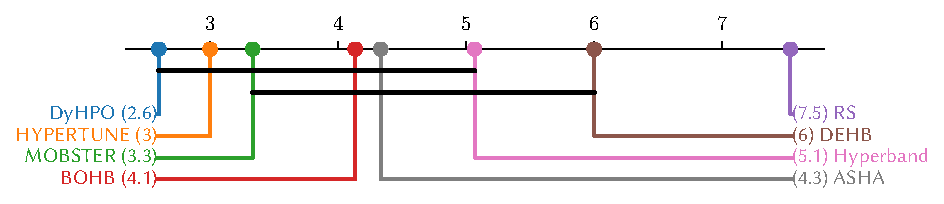
\includegraphics[scale=.75]{./img/tabular_exp/cd_diagram.pdf}
    \caption{Critical difference diagram for tabular benchmarks at the full budget. Average ranks are shown on the x-axis. Connected ranks via a bar indicate that performances are not significantly different ($p>0.05$).}
    \label{ci:tabular}
\end{figure}

For illustration purposes, we present the results of a single task in Figure~\ref{fig:parkinsons}. We provide the complete set of plots from all tasks in Appendix~\ref{ch:results_appendix}. We chose the fcnet-parkinsons task for the presentation because it allows us to show several general traits and performance of the algorithms. It is often the case in our experiments that random search is clearly behind all other algorithms, but it is catching up as the budget increases. We can also notice the fixed schedule of Hyperband. It takes Hyperband approximately 300 trials until it finally starts evaluating the first configuration fully. These delays hurt the early performance of Hyperband. In the case of FCNet with a maximal budget per configuration of 100 epochs, Hyperband should use approximately 25 full evaluations of budget per iteration. Therefore, it does not even finish the first iteration with our budget restriction. We can also notice that in the first bracket, the model-less Hyperband performs similarly to the model-based extensions. DEHB did not perform well in our experiments, it was often outperformed by model-less approaches. The performance of the most advanced methods was comparable. We cannot conclusively say that one is better than the other, as it often depends on the specific problem.

\begin{figure}
    \centering
    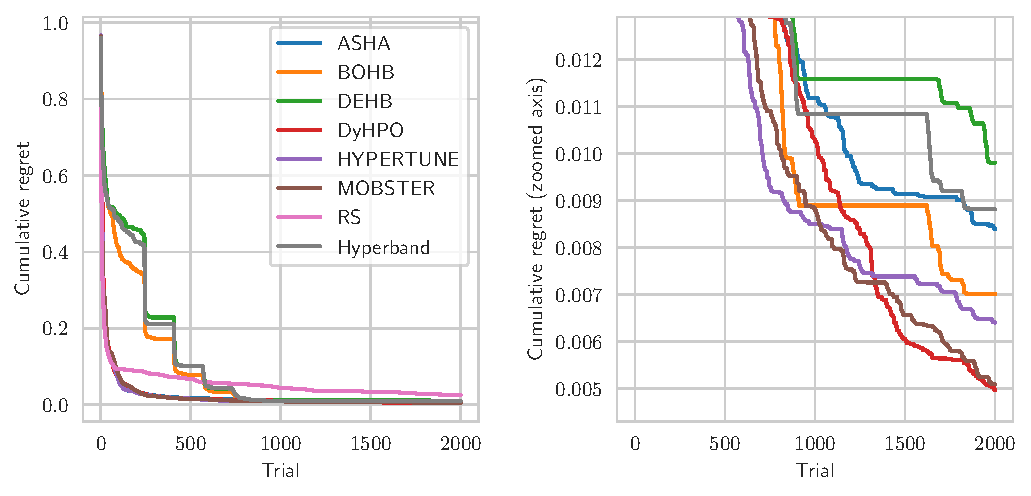
\includegraphics[scale=.75]{img/tabular_exp/fcnet-parkinsons_plot.pdf}
    \caption{The average regret over 30 runs on the fcnet-parkinsons task. On the right, we show the same results but zoomed in.}
    \label{fig:parkinsons}
\end{figure}

% Speedup factor
The key focus of this thesis is efficiency. We measure efficiency by comparing the algorithms to random search. We compute how much faster can the algorithms find a solution as good as random search has found after spending the whole budget. We call this measure the speedup factor and present the results in Table~\ref{tab:speedup}. The reported speedup factor is averaged over all benchmarks and repetitions. We assume a speedup is greater than one, which was broken for one dataset, where random search showed the best performance with a small margin. Because we do not have the data beyond the maximal budget, we have set the speedup factor to 1 in such cases. Nevertheless, the speedup factors are significant. Even the lowest reported value from any confidence interval is $3.39$ and the values of averages are around $6$ for the more advanced algorithms. The confidence intervals are overlapping for all pairs of algorithms, though.

\subfile{./tables/tab_results.tex}

% Overhead
We have seen that in terms of epochs, all advanced methods beat random search in efficiency. But that neglects the runtime, which could offset the gains. We examine the overhead in Figure~\ref{fig:overhead}. There are several things to note first. The overhead depends on the implementation. We compare all algorithms within the same framework on the same benchmark, but we have noticed there is an overhead of approximately 2 seconds when configurations change, both for a new configuration and a resumed configuration. DyHPO suffers from this kind of overhead the most because the used implementation pauses training after 2 epochs at most, even if the same configuration is immediately resumed again. That is why we see the steepest and almost linear line for DyHPO.\@ The methods based on Hyperband have the highest overhead in the beginning because they start with a bracket that tries the most configurations for the smallest budget. In the fcnet-naval example, a new configuration is sampled at each trial for the first 250 trials. From the comparison between ASHA and HyperTune, or ASHA and MOBSTER, we can see the overhead of the Bayesian surrogate model. We can notice that the slope of the overhead changes more with additional trials for the model-based algorithms than for ASHA, but the difference is not that large.
\begin{figure}
    \centering
    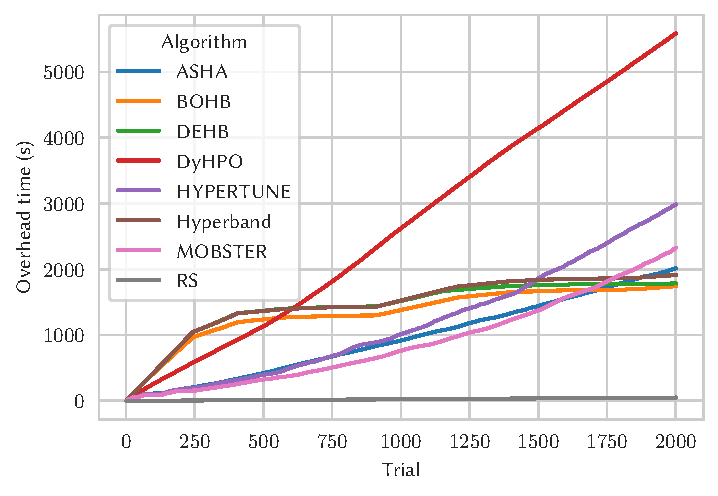
\includegraphics[scale=0.75]{./img/tabular_exp/overhead.pdf}
    \caption{Overhead on FCNet Naval benchmark.}
    \label{fig:overhead}
\end{figure}

% Heatmap
In order to estimate the reliability and consistency of the methods, we provide the heatmap of sample standard deviations (SD) in Figure~\ref{fig:heatmap}. The SDs are normalized across tasks because we are interested in a relative comparison between the algorithms, not in the actual magnitudes. We can see that random search has the largest SD in almost all tasks. Interestingly, it has the smallest SD in the lcbench-covertype tasks. After closer inspection of the results, one possible explanation might be that all algorithms struggle to consistently find a good solution. Although random search achieved the best SD, its results on that task were the worst by a large margin. In other words, its SD is probably low because it fails to find a good solution most of the time, unlike the other algorithms that are more successful. DyHPO even has the second-best SD on lcbench-covertype, and achieved the best results by a large margin.

The most pronounced differences between the worst and the best algorithms can be noticed in the FCNet tasks. Nevertheless, there are not many other obvious patterns in the data. HyperTune and MOBSTER seem to be the most consistent in FCNet tasks overall, and they also do well in NAS-Bench tasks, even if we consider the results. In LCBench tasks, DyHPO seems to be one of the most consistent algorithms on average, but its SD is high on the \textit{albert} and the \textit{christine} datasets. It might be the most useful to compare the average standard deviation across all tasks. DyHPO has the lowest mean SD, followed closely by ASHA, with HyperTune in third place. The other algorithms are also not far behind. DEHB is second to last, and random search is last.

\begin{figure}[H]
    \centering
    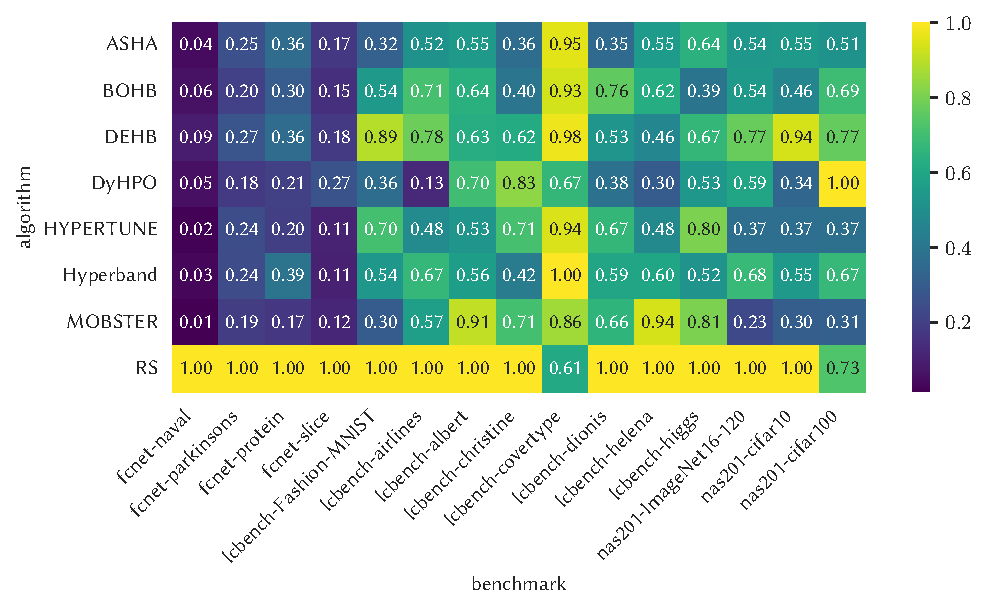
\includegraphics[scale=0.75]{img/tabular_exp/stds_heatmap.pdf}
    \caption{The heatmap of sample standard deviations of the best results found, averaged over 30 repetitions. The standard deviations are normalized for each task.}
    \label{fig:heatmap}
\end{figure}


\section{Real-world experiments results}

First, we present the combined results from all real-world experiments (Figure~\ref{fig:real_combined}). As anticipated, seven experiments are not enough for a~reliable statistical analysis. Nevertheless, the average ranks are still worth examining. The order of algorithms is very similar to the results from tabular benchmarks. The only difference at a \SI{100}{\percent} budget is that ASHA overtook BOHB on real-world tasks. Another thing to notice is that HyperTune performed better than DyHPO at a \SI{50}{\percent} budget, even though this difference is minor. Next, we will review the results for each experiment individually.


\begin{figure}[H]
    \begin{subfigure}{.5\textwidth}
        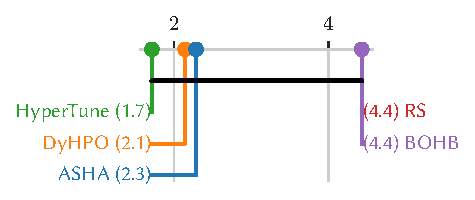
\includegraphics[width=.92\textwidth]{img/real_exp/cd_diagram_real_half.pdf}%
        \caption{At \SI{50}{\percent} budget.}%
        %\label{fig:second}
    \end{subfigure}%
    \begin{subfigure}{.5\textwidth}
        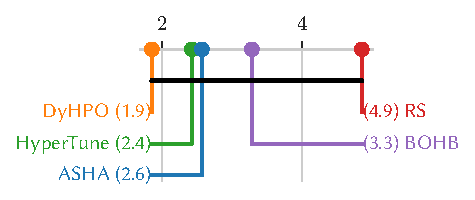
\includegraphics[width=.92\textwidth]{img/real_exp/cd_diagram_real.pdf}%
        \caption{At \SI{100}{\percent} budget.}%
        %\label{fig:first}
    \end{subfigure}%
\caption{Critical difference diagrams for real-world experiments at two budget levels. Average ranks are shown on the x-axis. All algorithms are connected via a bar, which indicates that performances are not significantly different ($p>0.05$).}
\label{fig:real_combined}
\end{figure}

%\subsection{Evaluation}
%\subsection{Experimental Setup}


%\begin{figure}[H]
%    \centering
%    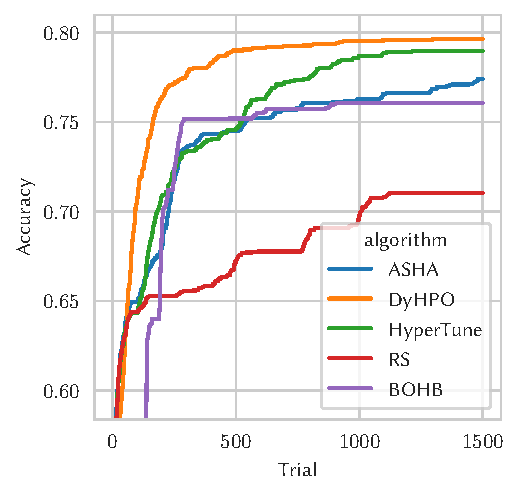
\includegraphics[scale=0.58]{img/real_exp/cifar10_simple_plot.pdf}
%    \caption{CNN network trained on CIFAR10 dataset for 20 full evaluations.}
%    \label{fig:cifar10}
%\end{figure}

%\subfile{./tables/cifar10_simple_results.tex}

%\subfile{./tables/cifar10_simple_results_short.tex}

%
%\begin{figure}[H]
%    \centering
%    \begin{minipage}[b]{2.5in}
%        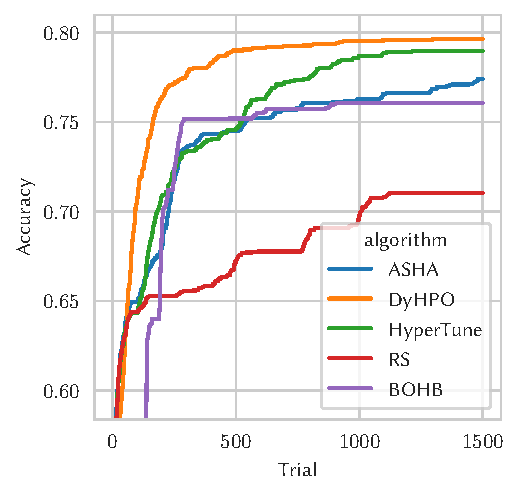
\includegraphics[width=\linewidth]{img/real_exp/cifar10_simple_plot.pdf}
%        \caption{Your Plot Caption}
%    \end{minipage}
%    \hfill
%    \begin{minipage}[b]{2.5in}
%        \input{./tables/cifar10_simple_results_short.tex}
%        \caption{Your Table Caption}
%    \end{minipage}
%\end{figure}
%

\subsubsection{1.\ cifar10-cnn}
In the first experiment, the differences between the algorithms are the most pronounced (see Figure~\ref{fig:simple_cifar}). Indeed, using the Kruskal-Wallis test we can reject the null hypothesis and conclude that there is a statistically significant difference in the medians of the groups at both budgets. Random search is far behind the other algorithms, especially early in the search. At full budget, some solutions found by random search get close to the better-performing algorithms, but not reliably. We use Dunn's test to reject the null hypothesis for random search and DyHPO, and random search and HyperTune at both budgets, concluding there is a statistically significant difference between the algorithms. DyHPO dominates the early stage of the search, especially when compared to ASHA and BOHB, which do not achieve at \SI{100}{\percent} of the budget results that DyHPO achieves at \SI{50}{\percent} of the budget. The differences between DyHPO and ASHA with BOHB are also statistically significant for both budgets. Finally, HyperTune is significantly better than BOHB at full budget.

\begin{figure}[H]
    \begin{subfigure}{.47\textwidth}
        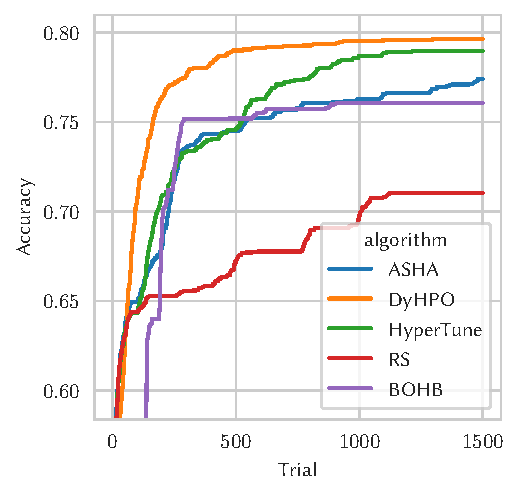
\includegraphics[height=\plotheight]{img/real_exp/cifar10_simple_plot.pdf}%
        \caption{Cumulative accuracy.}%
        %\label{fig:first}
    \end{subfigure}%
    \begin{subfigure}{.26\textwidth}
        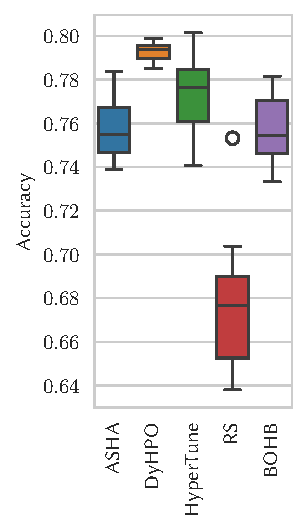
\includegraphics[height=\plotheight]{img/real_exp/cifar10_simple_boxplot_half.pdf}%
        \caption{At \SI{50}{\percent} budget.}%
        %\label{fig:second}
    \end{subfigure}%
    \begin{subfigure}{.26\textwidth}
        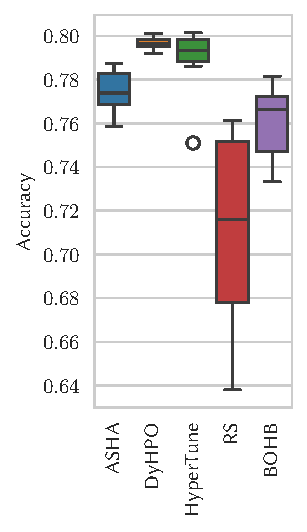
\includegraphics[height=\plotheight]{img/real_exp/cifar10_simple_boxplot_full.pdf}%
        \caption{At \SI{100}{\percent} budget.}%
        %\label{fig:second}
    \end{subfigure}%
\caption{Results of the cifar10-cnn experiment.}
\label{fig:simple_cifar}
\end{figure}

\subsubsection{2.\ cifar10-residual}
We can notice that residual CNN architecture performs much better than the simpler CNN architecture from the previous experiment, even very early in the search (see Figure~\ref{fig:resnet_cifar10}). On the other hand, the differences between hyperparameter optimization algorithms are small. A Kruskal-Wallis test resulted in a p-value of $0.51$ at a \SI{100}{\percent} budget and $0.20$ at a \SI{50}{\percent} budget, both of which are greater than the significance level of $0.05$. Therefore, we fail to reject the null hypothesis and conclude that there is no statistically significant difference in the medians of the groups at both budgets. With that said, BOHB achieved the best median and mean result on a full budget, even though not significantly better. Also, ASHA found a solution with over \SI{90}{\percent} accuracy in each run, which cannot be said for the other algorithms.

\begin{figure}[H]
    \begin{subfigure}{.47\textwidth}
        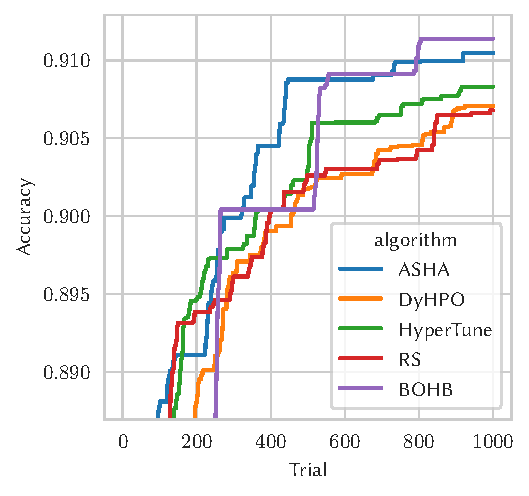
\includegraphics[height=\plotheight]{img/real_exp/cifar10_residual_plot.pdf}%
        \caption{Cumulative accuracy.}%
        %\label{fig:first}
    \end{subfigure}%
    \begin{subfigure}{.26\textwidth}
        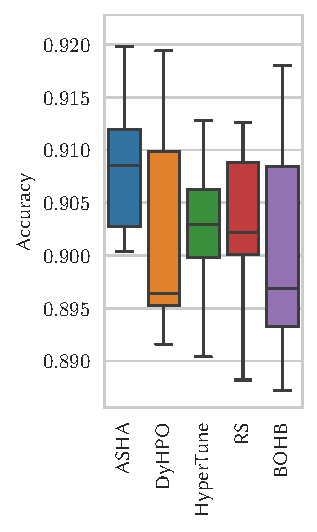
\includegraphics[height=\plotheight]{img/real_exp/cifar10_residual_boxplot_half.pdf}%
        \caption{At \SI{50}{\percent} budget.}%
        %\label{fig:second}
    \end{subfigure}%
    \begin{subfigure}{.26\textwidth}
        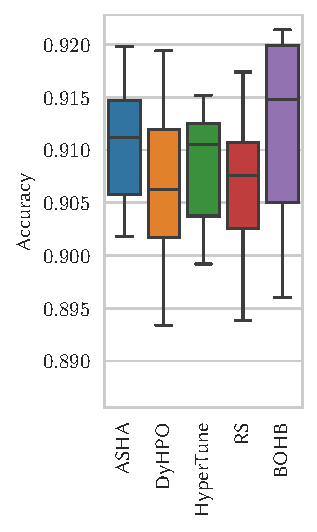
\includegraphics[height=\plotheight]{img/real_exp/cifar10_residual_boxplot_full.pdf}%
        \caption{At \SI{100}{\percent} budget.}%
        %\label{fig:second}
    \end{subfigure}%
\caption{Results of the cifar10-residual experiment.}
\label{fig:resnet_cifar10}
\end{figure}

\subsubsection{3.\ svhn-cnn}
Except for the dataset, this experiment is identical to the first experiment. The results of this experiment also resemble the results of the first experiment (see Figure~\ref{fig:simple_svhn}), but there are some differences. Most notably, DyHPO seemed to do better in the first experiment, and it is more in line with the other algorithms here. Kruskal-Wallis test rejects the null hypothesis for both budgets. Therefore, we follow up with Dunn's test. At \SI{50}{\percent} of the budget, all algorithms significantly outperform random search. By~contrast, the performance of other algorithms seems to be almost identical at a \SI{50}{\percent} budget. At full budget, the null hypothesis cannot be rejected for random search with ASHA, and random search with BOHB.\@ On the other hand, HyperTune and DyHPO did perform significantly better than random search. There is a statistically significant difference between DyHPO and BOHB, too.\@ We can also notice that DyHPO and HyperTune were both more consistent in finding a good solution than other algorithms.

\begin{figure}[H]
    \begin{subfigure}{.47\textwidth}
        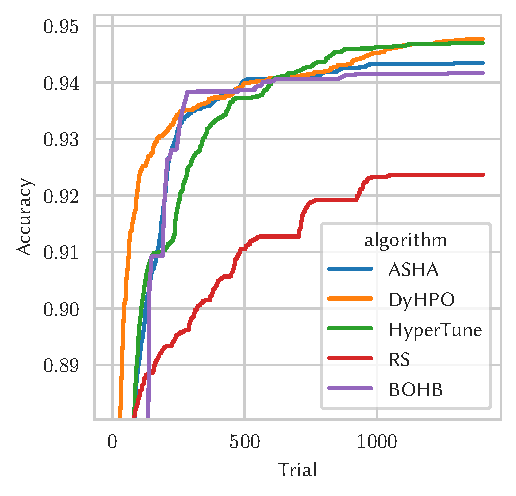
\includegraphics[height=\plotheight]{img/real_exp/svhn_simple_plot.pdf}%
        \caption{Cumulative accuracy.}%
        %\label{fig:first}
    \end{subfigure}%
    \begin{subfigure}{.26\textwidth}
        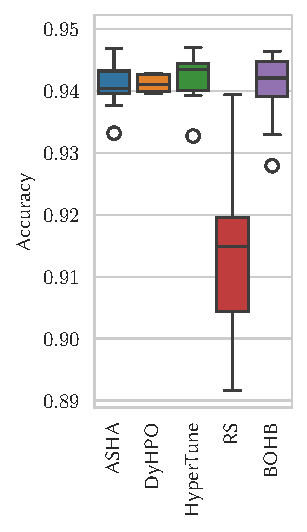
\includegraphics[height=\plotheight]{img/real_exp/svhn_simple_boxplot_half.pdf}%
        \caption{At \SI{50}{\percent} budget.}%
        %\label{fig:second}
    \end{subfigure}%
    \begin{subfigure}{.26\textwidth}
        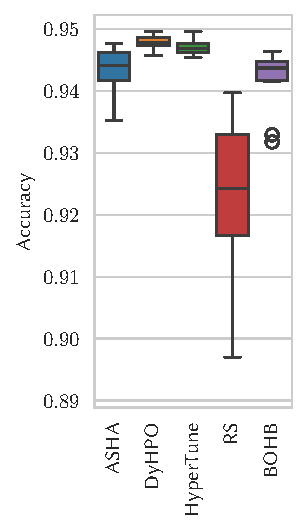
\includegraphics[height=\plotheight]{img/real_exp/svhn_simple_boxplot_full.pdf}%
        \caption{At \SI{100}{\percent} budget.}%
        %\label{fig:second}
    \end{subfigure}%
\caption{Results of the svhn-cnn experiment.}
\label{fig:simple_svhn}
\end{figure}


\subsubsection{4.\ svhn-residual}
Again, we see the importance of choosing the right architecture if we compare the results between this and the previous experiment. The results of a random search in this experiment (see Figure~\ref{fig:resnet_svhn}) start where the best networks from the previous experiment end. Kruskal-Wallis test results in p-values far below the significance level for both budgets, so we reject both null hypotheses. Dunn's pairwise comparison test points out significant differences between random search and all other algorithms on both budgets, except for ASHA at a \SI{50}{\percent} budget and BOHB at a \SI{100}{\percent} budget. The null hypothesis cannot be rejected for the other pairwise comparisons, though. DyHPO seems to offer the best anytime performance, as well as the full-budget performance, albeit with a small margin. Other algorithms are very close behind DyHPO.\@ Again, random search has the largest variance, especially on half of the budget.

\begin{figure}[H]
    \begin{subfigure}{.47\textwidth}
        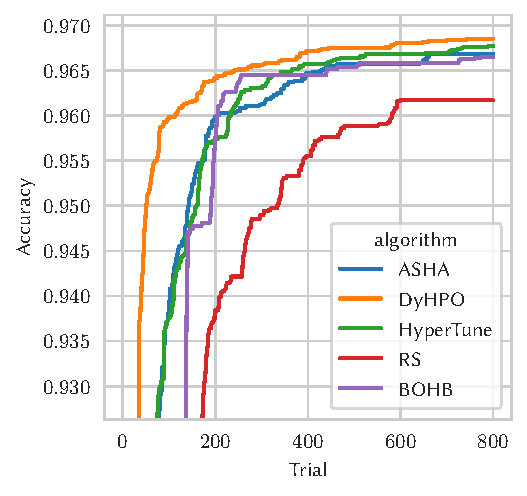
\includegraphics[height=\plotheight]{img/real_exp/svhn_residual_plot.pdf}%
        \caption{Cumulative accuracy.}%
        %\label{fig:first}
    \end{subfigure}%
    \begin{subfigure}{.26\textwidth}
        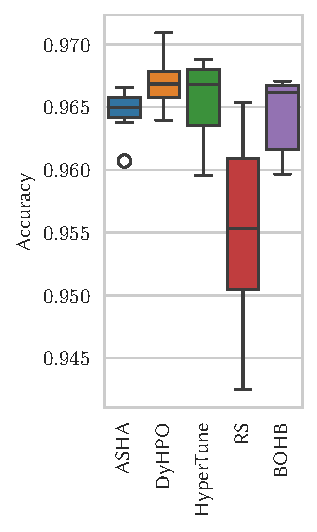
\includegraphics[height=\plotheight]{img/real_exp/svhn_residual_boxplot_half.pdf}%
        \caption{At \SI{50}{\percent} budget.}%
        %\label{fig:second}
    \end{subfigure}%
    \begin{subfigure}{.26\textwidth}
        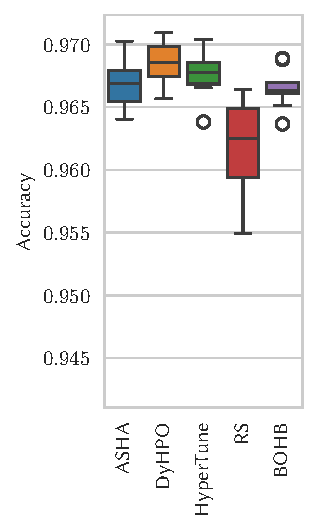
\includegraphics[height=\plotheight]{img/real_exp/svhn_residual_boxplot_full.pdf}%
        \caption{At \SI{100}{\percent} budget.}%
        %\label{fig:second}
    \end{subfigure}%
\caption{Results of the svhn-residual experiment.}
\label{fig:resnet_svhn}
\end{figure}


\subsubsection{5.\ ptbxl-rnn}
% NO significant differences at both budgets
We conducted a Kruskal-Wallis test, which resulted in p-values $0.13$ and $0.36$ at a full budget, and a half budget respectively. Therefore, we cannot reject the null hypothesis for both budgets. All methods achieved very similar results (see Figure~\ref{fig:rnn_ptbxl}); and it is not possible to tell if any method is better than the other. We can notice that the solutions found on half of the budget are only marginally worse than solutions found on the full budget. Also, the variance of the results is similar for all algorithms including random search. If any differences can be found, DyHPO has a slightly larger variance than other algorithms on both budgets.

\begin{figure}[H]
    \begin{subfigure}{.47\textwidth}
        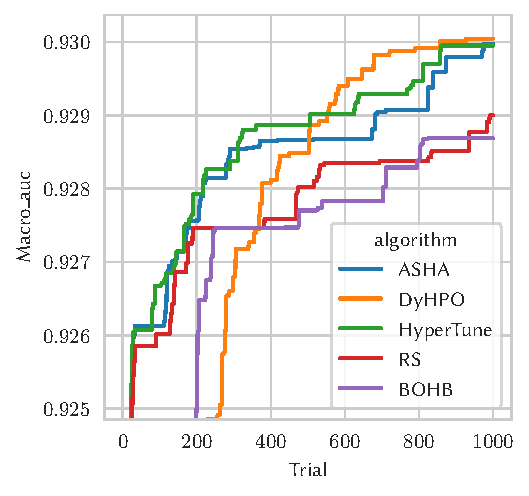
\includegraphics[height=\plotheight]{img/real_exp/ptbxl_rnn_plot.pdf}%
        \caption{Cumulative averaged ROC AUC score.}%
        %\label{fig:first}
    \end{subfigure}%
    \begin{subfigure}{.26\textwidth}
        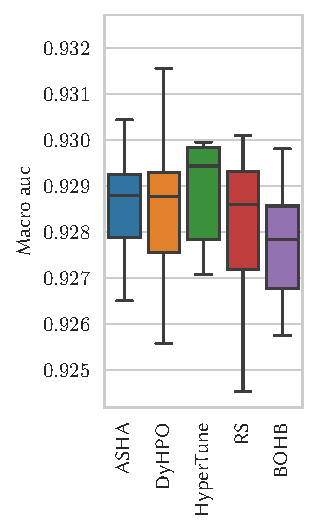
\includegraphics[height=\plotheight]{img/real_exp/ptbxl_rnn_boxplot_half.pdf}%
        \caption{At \SI{50}{\percent} budget.}%
        %\label{fig:second}
    \end{subfigure}%
    \begin{subfigure}{.26\textwidth}
        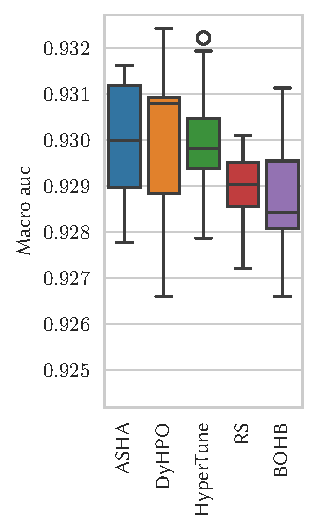
\includegraphics[height=\plotheight]{img/real_exp/ptbxl_rnn_boxplot_full.pdf}%
        \caption{At \SI{100}{\percent} budget.}%
        %\label{fig:second}
    \end{subfigure}%
\caption{Results of the ptbxl-rnn experiment.}
\label{fig:rnn_ptbxl}
\end{figure}


\subsubsection{6.\ ptbxl-xResnet1d}
% NO differences at 100, some differences at 50
In spite of the fact that xResnet1d was the best-performing architecture on the PTB-XL dataset according to the literature~\cite{strodthoff2020deep}, it seems to perform a little worse than RNN in our experiments (see Figure~\ref{fig:xresnet_ptbxl}). There is a small overlap between the results of the two architectures, though. Kruskal-Wallis test rejected the null hypothesis on both budgets. However, the follow-up Dunn's test did not find any significant differences at the full budget. At a \SI{50}{\percent} of the budget, the null hypothesis can be rejected for many pairs. Random search performed significantly worse than HyperTune and ASHA.\@ HyperTune and ASHA are indistinguishable statistically, but both performed better than all other algorithms at a \SI{50}{\percent} budget. One more thing to note is that random search has a much larger variance than other methods on half of the budget.

\begin{figure}[H]
    \begin{subfigure}{.47\textwidth}
        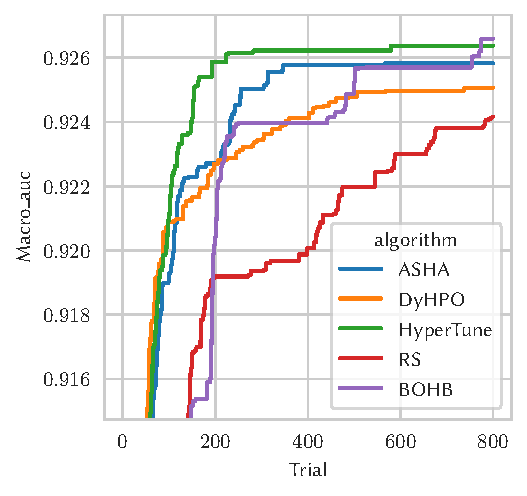
\includegraphics[height=\plotheight]{img/real_exp/ptbxl_xResNet1d_plot.pdf}%
        \caption{Cumulative averaged ROC AUC score.}%
        %\label{fig:first}
    \end{subfigure}%
    \begin{subfigure}{.26\textwidth}
        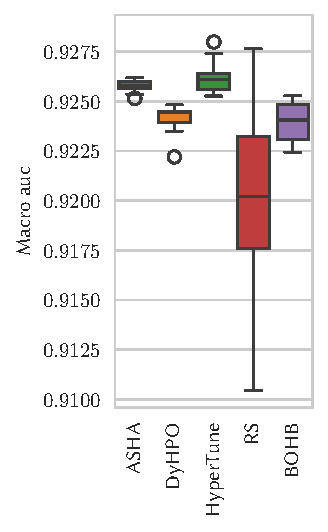
\includegraphics[height=\plotheight]{img/real_exp/ptbxl_xResNet1d_boxplot_half.pdf}%
        \caption{At \SI{50}{\percent} budget.}%
        %\label{fig:second}
    \end{subfigure}%
    \begin{subfigure}{.26\textwidth}
        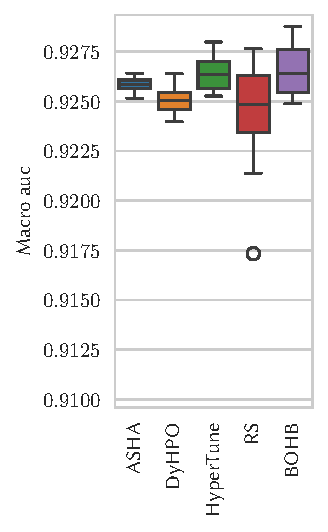
\includegraphics[height=\plotheight]{img/real_exp/ptbxl_xResNet1d_boxplot_full.pdf}%
        \caption{At \SI{100}{\percent} budget.}%
        %\label{fig:second}
    \end{subfigure}%
\caption{Results of the ptbxl-xResnet1d experiment.}
\label{fig:xresnet_ptbxl}
\end{figure}


\subsubsection{7.\ xray-densenet}
% RS DyHpo different at full budget, NO differences at 50%
The last experiment was performed on the ChestX-ray14 dataset. The p-values of Kruskal-Wallis tests are $0.02$ at a \SI{100}{\percent} budget, and $0.09$ at a \SI{100}{\percent} budget. Therefore, we can reject the null hypothesis at the full budget only. Dunn's test found a significant difference only for the DyHPO and random search pair, where DyHPO performed significantly better than random search. The other results are very close (see Figure~\ref{fig:densenet_chestx}). ASHA seems to be slightly better at half of the budget than the other algorithms except for DyHPO, but then it barely improves until the end. The random search did well in this experiment, too, considering that it is comparable to the other algorithms.

\begin{figure}[H]
    \begin{subfigure}{.47\textwidth}
        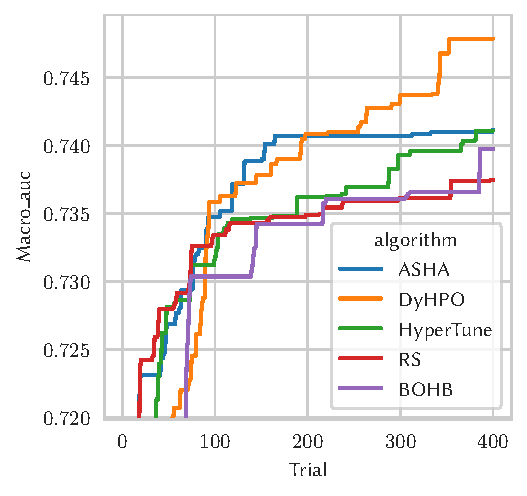
\includegraphics[height=\plotheight]{img/real_exp/xray_densenet_plot.pdf}%
        \caption{Cumulative averaged ROC AUC score.}%
        %\label{fig:first}
    \end{subfigure}%
    \begin{subfigure}{.26\textwidth}
        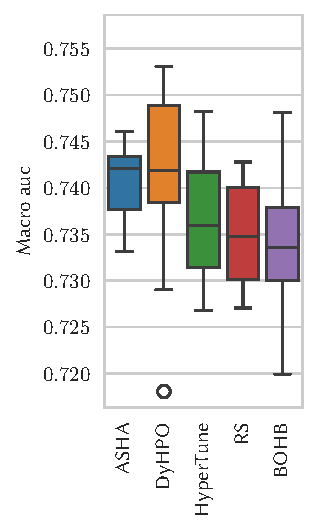
\includegraphics[height=\plotheight]{img/real_exp/xray_densenet_boxplot_half.pdf}%
        \caption{At \SI{50}{\percent} budget.}%
        %\label{fig:second}
    \end{subfigure}%
    \begin{subfigure}{.26\textwidth}
        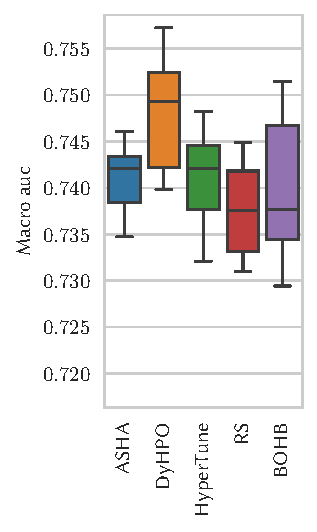
\includegraphics[height=\plotheight]{img/real_exp/xray_densenet_boxplot_full.pdf}%
        \caption{At \SI{100}{\percent} budget.}%
        %\label{fig:second}
    \end{subfigure}%
\caption{Results of the xray-densenet experiment.}
\label{fig:densenet_chestx}
\end{figure}


% \clearpage
\section{Discussion} % Interpret and explain my results

% Restate your research problem and research questions

% Summary of key findings

    % the data suggest that..
    % the data support/oppose the theory that..
    % the analysis identifies..

% Interpretation of results
% More detailed findigs

% Speedup factor and inconsistency
The data suggest advanced algorithms can find a good solution much faster than random search. In tabular experiments, the average speedup factor of algorithms over random search was approximately in the range of $4.5$ for DEHB and Hyperband, to $7$ for DyHPO.\@ Meaning that DyHPO found a solution as good as the random search, but only using a $1/7$th of the budget on average. There was just a single task out of the fifteen, where random search was comparable to the other algorithms. Another important thing to consider is that random search is less consistent. We have observed that the spread of the results can be many times larger for random search, in addition to usually being worse on average. The data suggest that if there is just one opportunity to optimize the hyperparameters or the budget is very limited, a random search will not find a good solution reliably.
% Did we?

% Real-world architectures - large differences on CNN
The results from real-world experiments were more diverse. We have seen the largest differences between algorithms on the simplest architecture. We think that the hyperparameters probably had a larger effect on the small CNN network than on the large and complex networks, because the large networks have a large capacity overhead and also use techniques like residual connections to make learning easier. Take the xResnet1d as an example. From the individual runs we have found that all three network sizes were able to achieve over $0.925$ ROC AUC score, which is very close to the best achieved result, suggesting that the size of the network alone did not have much influence over the performance.

We have found no statistically significant differences between algorithms in cifar10-residual and ptbxl-rnn experiments, which illustrates that some tasks might not even benefit from an advanced hyperparameter tuning algorithm. Nevertheless, there were significant differences in all the other experiments. Most often, random search performed significantly worse than DyHPO and HyperTune. Since the ranking of the algorithms is mostly consistent with ranking in tabular experiments, we think that more differences could be found; we just do not have enough data to support it.

% Mention healthcare datasets


% Comparison with previous work

% Maybe todo? Practical implications


% Recommendations
From the research, we have several recommendations. We recommend using random search in the exploratory phase when the goal is to gain as much insight into the problem as possible. If the goal is to optimize hyperparameters efficiently, we think it is better to avoid random search. Especially ASHA sped up the search almost as much as the best algorithms without any of the downsides. It is easy to implement, parallelization is simple, and it does not even require checkpointing in the stopping variant. Moreover, the lack of a model makes it robust, as the new suggestions are always going to be randomly sampled. If the extra efficiency is needed, we recommend either DyHPO or HyperTune. DyHPO seemed to perform a little better overall, but it pauses and resumes trials much more often. Therefore, if resuming trials is expensive, we would recommend HyperTune over DyHPO.\@

We also want to point out that while the original goal was to implement a new method based on the findings of our experiments, in the end, we decided to focus exclusively on the experimental comparison, as we found out that there are no independent comparisons in the literature that we are aware of. Such comparisons are needed to uncover the strengths and weaknesses of the existing methods before new methods can be designed. Moreover, this kind of research helps practitioners pick the right algorithm, as it provides new data and eliminates the need to go through multiple articles to understand different methods and their performance.


% One of the barriers to the widespread adoption of hyperparameter optimization algorithms is the lack of empirical evidence to decide which algorithm to choose. We performed a set of experiments, both on tabular benchmarks and on real-world problems, in order to provide more data and to help practitioners with the decision of choosing a suitable hyperparameter optimization algorithm for the task at hand.


\chapwithtoc{Conclusion}

% Where in the research map is my thesis - mention some work that has been done
%       - on HPO in general
%       - on comparisons
% To what extent did we responded to the gap in research


% We did perform quite a lot of new experiments, more than would be possible on just a single personal computer.

%  One such example is DyHPO, which dynamically selects the most promising configuration to evaluate, potentially after each training epoch.

Numerous hyperparameter optimization algorithms are available for deployment, many of which focus on efficiency through multi-fidelity evaluations. However, selecting the right method can be challenging, especially when most of the performance comparisons available are from the original research papers that introduce the algorithms. Moreover, the comparisons are often not very detailed, and authors choose which tasks and methods to include. In this thesis, we conducted experiments to provide independent and varied comparisons of the state-of-the-art algorithms to help practitioners make better decisions.

We found that by using an advanced algorithm, it is often possible to obtain a solution comparable to a solution found by random search, but using just a fraction of the budget. On tabular experiments, DyHPO achieved an average speedup factor of $6.92$ compared to random search. DyHPO proved to be one of the best algorithms in the comparison, achieving the best average rank on both tabular and real-world experiments, closely followed by HyperTune. One thing to note is that DyHPO can have a large overhead depending on the implementation. The results of the real-world experiments were more varied, which is why including diverse tasks and architectures in comparisons is needed. We did not find any major discrepancies between tabular and real-world experiments, suggesting that tabular benchmarks still provide a good general estimate of performance.

However, some limitations are worth noting. Most importantly, the data obtained from the real-world experiments were noisy, and 10 repetitions were insufficient to uncover more statistically supported findings. Moreover, the problems solved in the real-world experiments were still orders of magnitude simpler than some problems currently solved by machine learning, even though we included more recent architectures and often larger search spaces than tabular benchmarks. Future work should therefore focus on extending the diversity of tasks, e.g.\ by including NLP or reinforcement learning tasks; and performing more repetitions for more reliable results. Moreover, creating a new set of tabular benchmarks with more recent problems would also be valuable, as tabular benchmarks are useful not only for comparisons but more importantly for the development of new algorithms.


% Considering the field of hyperparameter optimization more broadly, we think that subsampling is an underexplored area of research as a means to improve the efficiency of the search. The existing methods did not catch up though, probably because they introduce yet another barrier for practitioners --- the datasets have to support subsampling. Nevertheless, we think that experimenting with coresets or some other way of subsampling shows a potential for another speed-up of the hyperparameter optimization.
\include{bibliography}

\appendix
%\chapter{Benchmarks specifications}
\label{ch:specs_appendix}

\section{Tabular}

% \subfile{./tables/tabular_summary.tex}


% \begin{table}[H]
% \begin{tabular}{lc}
%     \toprule
%     Hyperparameter & Values \\
%     \midrule
%     Batch size & $\{16,\ldots , 512\}$ \\
%     Learning rate & $\interval{1\mathrm{e}{-4}}{1\mathrm{e}{-1}}$ \\
%     Momentum & $\interval{0.1}{0.99}$ \\
%     Weight decay & $\interval{1\mathrm{e}{-5}}{1\mathrm{e}{-1}}$ \\
%     Layers & $\{1,2,3,4,5\}$ \\
%     Max units/layer & $\{64, \ldots , 1024\}$ \\
%     Dropout & $\interval{0.0}{1.0}$ \\
%     \bottomrule
%     \end{tabular}
%     \caption{LCBench hyperparameter values}
%     \label{tab:lc}
% \end{table}


% \begin{table}[H]
%     \centering
% \begin{tabular}{lc}
%     \toprule
%     Hyperparameter & Values \\
%     \midrule
%     Learning rate & $\{0.0005, 0.001, 0.005, 0.01, 0.05, 0.1\}$ \\
%     Batch size & $\{8, 16, 32, 64\}$ \\
%     LR schedule & $\{\text{cosine}, \text{fix} \}$ \\
%     Activation L1 & $\{\text{relu}, \text{tanh} \}$ \\
%     Activation L2 & $\{\text{relu}, \text{tanh} \}$ \\
%     L1 size & $\{8, 16, 32, 64, 128, 256, 512\}$ \\
%     L2 size & $\{8, 16, 32, 64, 128, 256, 512\}$ \\
%     Dropout L1 & $\{0.0, 0.3, 0.6\}$ \\
%     Dropout L2 & $\{0.0, 0.3, 0.6\}$ \\
%     \bottomrule
%     \end{tabular}
%     \caption{FCNet hyperparameter values}
%     \label{tab:fcnet}
% \end{table}

%\clearpage % Flushes float\s

\section{Real-world}

% tab:real_bench_summary















\chapter{Additional figures}
\label{ch:results_appendix}

\section{Tabular}

%Tabular benchmarks for joint architecture and hyperparameter optimization. Klein, A. and Hutter, F. 2019.
\begin{figure}[H]
    \centering
    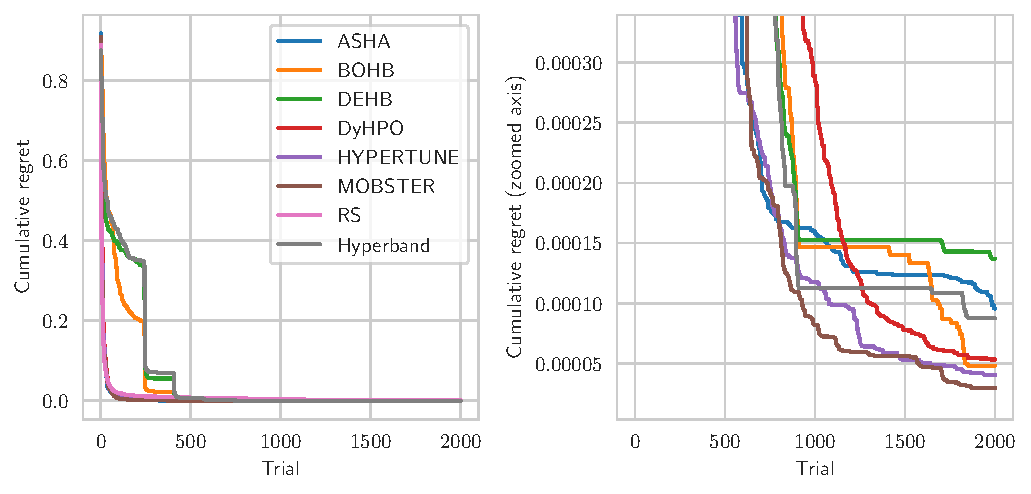
\includegraphics[scale=0.65]{img/tabular_exp/fcnet-naval_plot.pdf}
    \caption{Results of the fcnet-naval experiment.}
    %\label{}
\end{figure}

\begin{figure}[H]
    \centering
    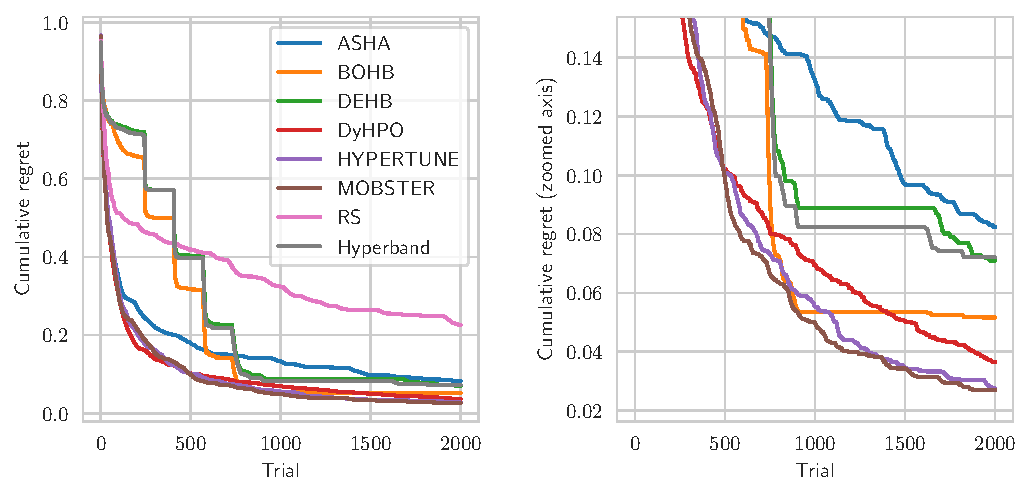
\includegraphics[scale=0.65]{img/tabular_exp/fcnet-protein_plot.pdf}
    \caption{Results of the fcnet-protein experiment.}
    %\label{}
\end{figure}


\begin{figure}[H]
    \centering
    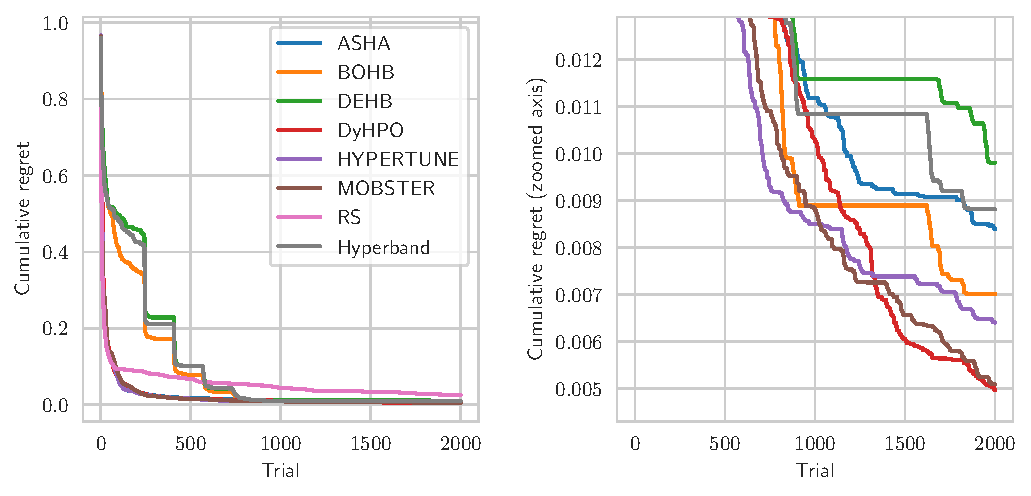
\includegraphics[scale=0.65]{img/tabular_exp/fcnet-parkinsons_plot.pdf}
    \caption{Results of the fcnet-parkinsons experiment.}
    %\label{}
\end{figure}

\begin{figure}[H]
    \centering
    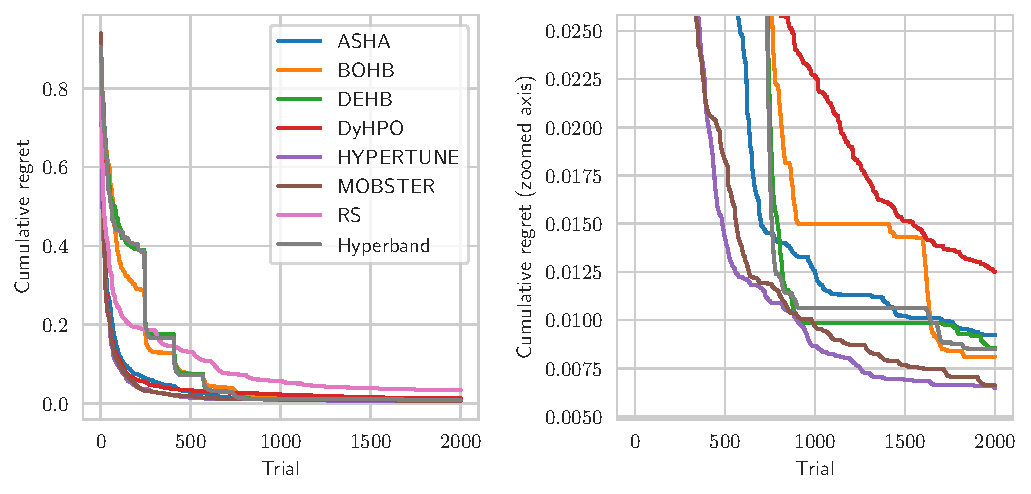
\includegraphics[scale=0.65]{img/tabular_exp/fcnet-slice_plot.pdf}
    \caption{Results of the fcnet-slice experiment.}
    %\label{}
\end{figure}




% NAS-Bench-201: Extending the scope of reproducible neural architecture search. Dong, X. and Yang, Y. 2020.
\begin{figure}[H]
    \centering
    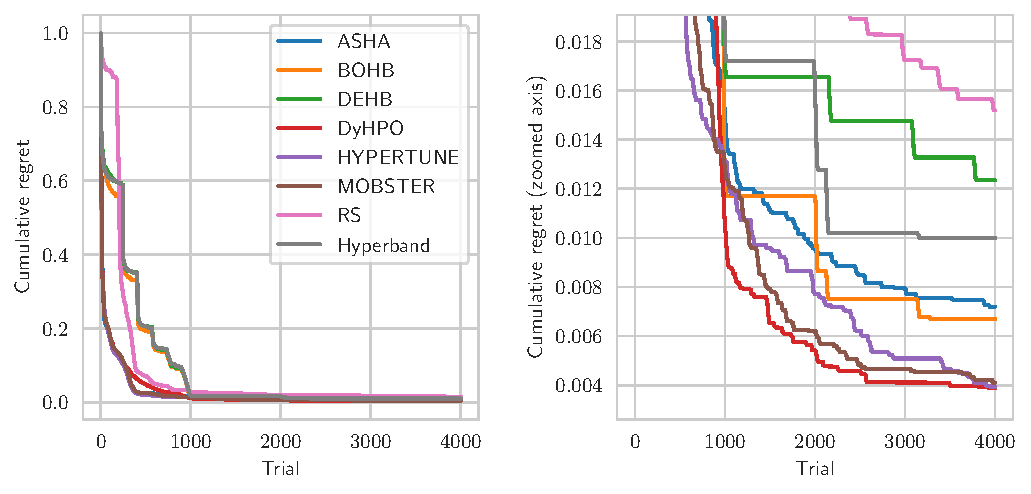
\includegraphics[scale=0.65]{img/tabular_exp/nas201-cifar10_plot.pdf}
    \caption{Results of the nas201-cifar10 experiment.}
    %\label{}
\end{figure}

\begin{figure}[H]
    \centering
    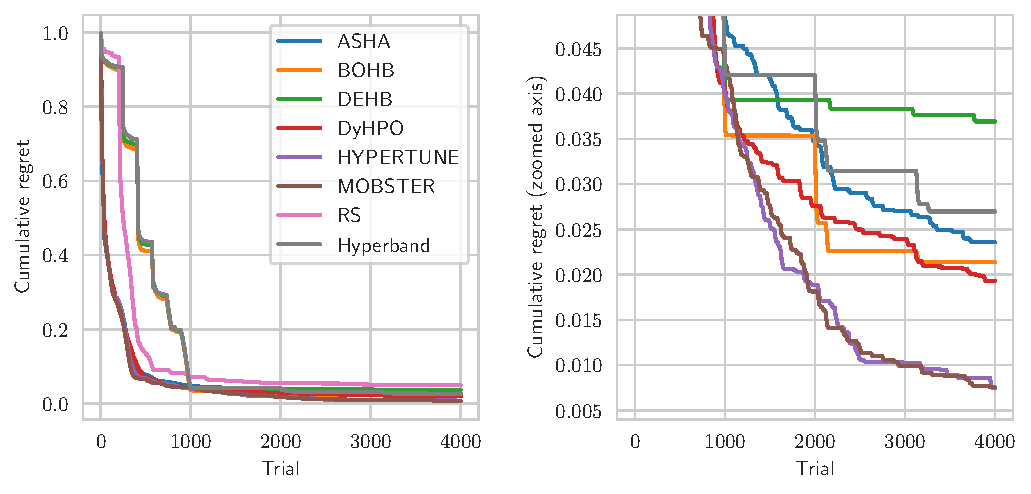
\includegraphics[scale=0.65]{img/tabular_exp/nas201-cifar100_plot.pdf}
    \caption{Results of the nas201-cifar100 experiment.}
    %\label{}
\end{figure}

\begin{figure}[H]
    \centering
    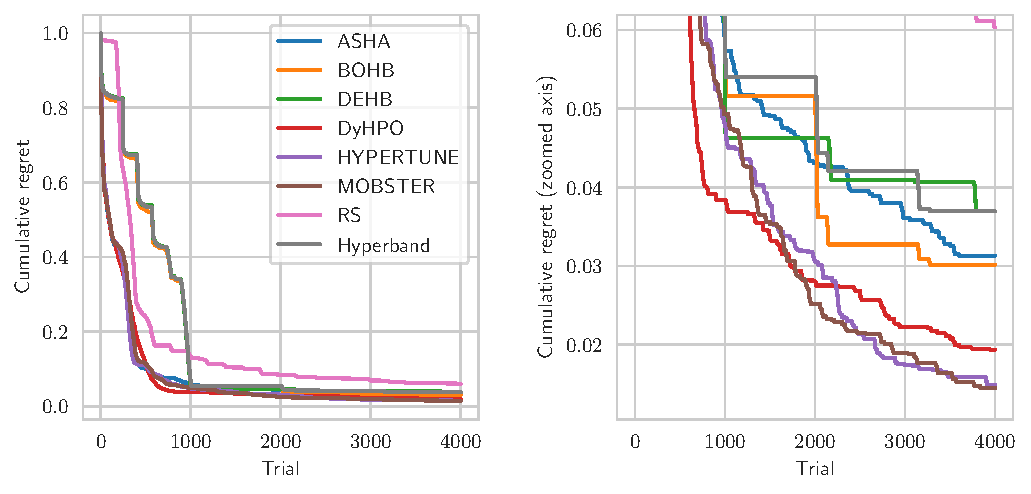
\includegraphics[scale=0.65]{img/tabular_exp/nas201-ImageNet16-120_plot.pdf}
    \caption{Results of the nas201-ImageNet16-120 experiment.}
    %\label{}
\end{figure}

%Reference: Auto-PyTorch: Multi-Fidelity MetaLearning for Efficient and Robust AutoDL. Lucas Zimmer, Marius Lindauer, Frank Hutter. 2020.
\begin{figure}[H]
    \centering
    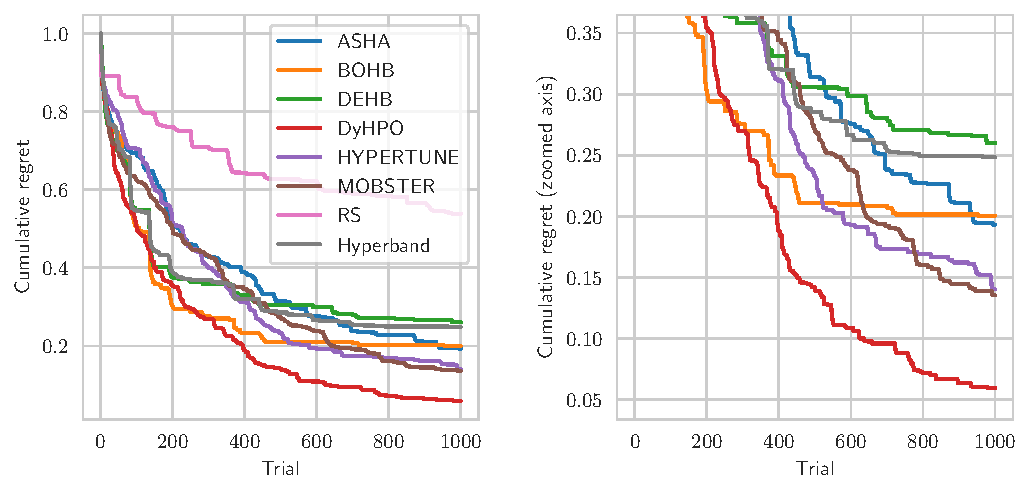
\includegraphics[scale=0.65]{img/tabular_exp/lcbench-airlines_plot.pdf}
    \caption{Results of the lcbench-airlines experiment.}
    %\label{}
\end{figure}

\begin{figure}[H]
    \centering
    \includegraphics[scale=0.65]{img/tabular_exp/lcbench-albert_plot.pdf}
    \caption{Results of the lcbench-albert experiment.}
    %\label{}
\end{figure}

\begin{figure}[H]
    \centering
    \includegraphics[scale=0.65]{img/tabular_exp/lcbench-Fashion-MNIST_plot.pdf}
    \caption{Results of the lcbench-Fashion-MNIST experiment.}
    %\label{}
\end{figure}

\begin{figure}[H]
    \centering
    \includegraphics[scale=0.65]{img/tabular_exp/lcbench-covertype_plot.pdf}
    \caption{Results of the lcbench-covertype experiment.}
    %\label{}
\end{figure}

\begin{figure}[H]
    \centering
    \includegraphics[scale=0.65]{img/tabular_exp/lcbench-christine_plot.pdf}
    \caption{Results of the lcbench-christine experiment.}
    %\label{}
\end{figure}

\begin{figure}[H]
    \centering
    \includegraphics[scale=0.65]{img/tabular_exp/lcbench-higgs_plot.pdf}
    \caption{Results of the lcbench-higgs experiment.}
    %\label{}
\end{figure}

\begin{figure}[H]
    \centering
    \includegraphics[scale=0.65]{img/tabular_exp/lcbench-dionis_plot.pdf}
    \caption{Results of the lcbench-dionis experiment.}
    %\label{}
\end{figure}

\begin{figure}[H]
    \centering
    \includegraphics[scale=0.65]{img/tabular_exp/lcbench-helena_plot.pdf}
    \caption{Results of the lcbench-helena experiment.}
    %\label{}
\end{figure}


\section{Real-world}


\begin{figure}[H]
    \centering
    \includegraphics[scale=0.65]{img/real_exp/cifar10_simple_regret_plot.pdf}
    \caption{Results of the cifar10-cnn experiment.}
    \label{fig:cifar10_simple}
\end{figure}

\begin{figure}[H]
    \centering
    \includegraphics[scale=0.65]{img/real_exp/cifar10_residual_regret_plot.pdf}
    \caption{Results of the cifar10-residual experiment.}
    \label{fig:cifar10_residual}
\end{figure}

\begin{figure}[H]
    \centering
    \includegraphics[scale=0.65]{img/real_exp/svhn_simple_regret_plot.pdf}
    \caption{Results of the svhn-cnn experiment.}
    \label{fig:svhn_simple}
\end{figure}

\begin{figure}[H]
    \centering
    \includegraphics[scale=0.65]{img/real_exp/svhn_residual_regret_plot.pdf}
    \caption{Results of the svhn-residual experiment.}
    \label{fig:svhn_residual}
\end{figure}


\begin{figure}[H]
    \centering
    \includegraphics[scale=0.65]{img/real_exp/ptbxl_rnn_regret_plot.pdf}
    \caption{Results of the ptbxl-rnn experiment.}
    \label{fig:ptbxl_rnn}
\end{figure}

\begin{figure}[H]
    \centering
    \includegraphics[scale=0.65]{img/real_exp/ptbxl_xResNet1d_regret_plot.pdf}
    \caption{Results of the ptbxl-xResnet1d experiment.}
    \label{fig:ptbxl_xresnet}
\end{figure}

\begin{figure}[H]
    \centering
    \includegraphics[scale=0.65]{img/real_exp/xray_densenet_regret_plot.pdf}
    \caption{Results of the xray-densenet experiment.}
    \label{fig:xray_densenet}
\end{figure}


% if your attachments are complicated, describe them in a separate appendix
%\include{attachments}

%\openright
\end{document}
